\documentclass[10pt,a4paper]{beamer}
\usepackage[latin1]{inputenc}
\usepackage[spanish]{babel}
\usepackage[T1]{fontenc}
\usepackage{amsmath}
\usepackage{amsfonts}
\usepackage{amssymb}
\usepackage{graphicx}
\usepackage{beamerthemesplit}
\usepackage{float}
\usepackage{multirow}
\usepackage{multicol}
\usepackage{url}
\usepackage{ragged2e}
\usepackage{array}
\usepackage{latexsym}
\usepackage{subfigure}
\usepackage{timing}
\usepackage{url}

\setbeamertemplate{footline}[frame number]
\setbeamertemplate{bibliography item}[text]
%\setbeamertemplate{subsubsection in sidebar shaded}
%{\tableofcontents[subsubsectionstyle=hide]}

%\usetheme{Montpellier}
\usetheme{Warsaw}
\decimalpoint
\renewcommand{\contentsname}{Contenido}

\begin{document}

\title{Integraci�n sem�ntica de \\ los recursos de informaci�n en \\ una memoria corporativa}
\author{Erik Alarc�n Zamora}
\date{Enero 2014. M�xico, D.F.}

\begin{frame}
\titlepage
\centering
Asesores:\\ Dra. Reyna Carolina Medina Ram�rez \\Dr. H�ctor P�rez Urbina
\\
\end{frame}
\begin{frame}
\frametitle{Contenido}
\setcounter{tocdepth}{1}  
\begin{scriptsize}\tableofcontents[]\end{scriptsize}
\end{frame}
\section{Contexto y motivaci�n}

\subsection{Memoria corporativa}
\begin{frame}
	\frametitle{Memoria Corporativa}
	%%%%%%%%%%%%%%%%%%%%%%%
	\begin{block}{Definici�n}
	\justifying 
	La representaci�n expl�cita, t�cita, consistente y persistente del conocimiento de una organizaci�n. \cite{Ontoinra2002}
	\end{block}
	
	\begin{figure}[htbp]
	\centering
	\subfigure{
	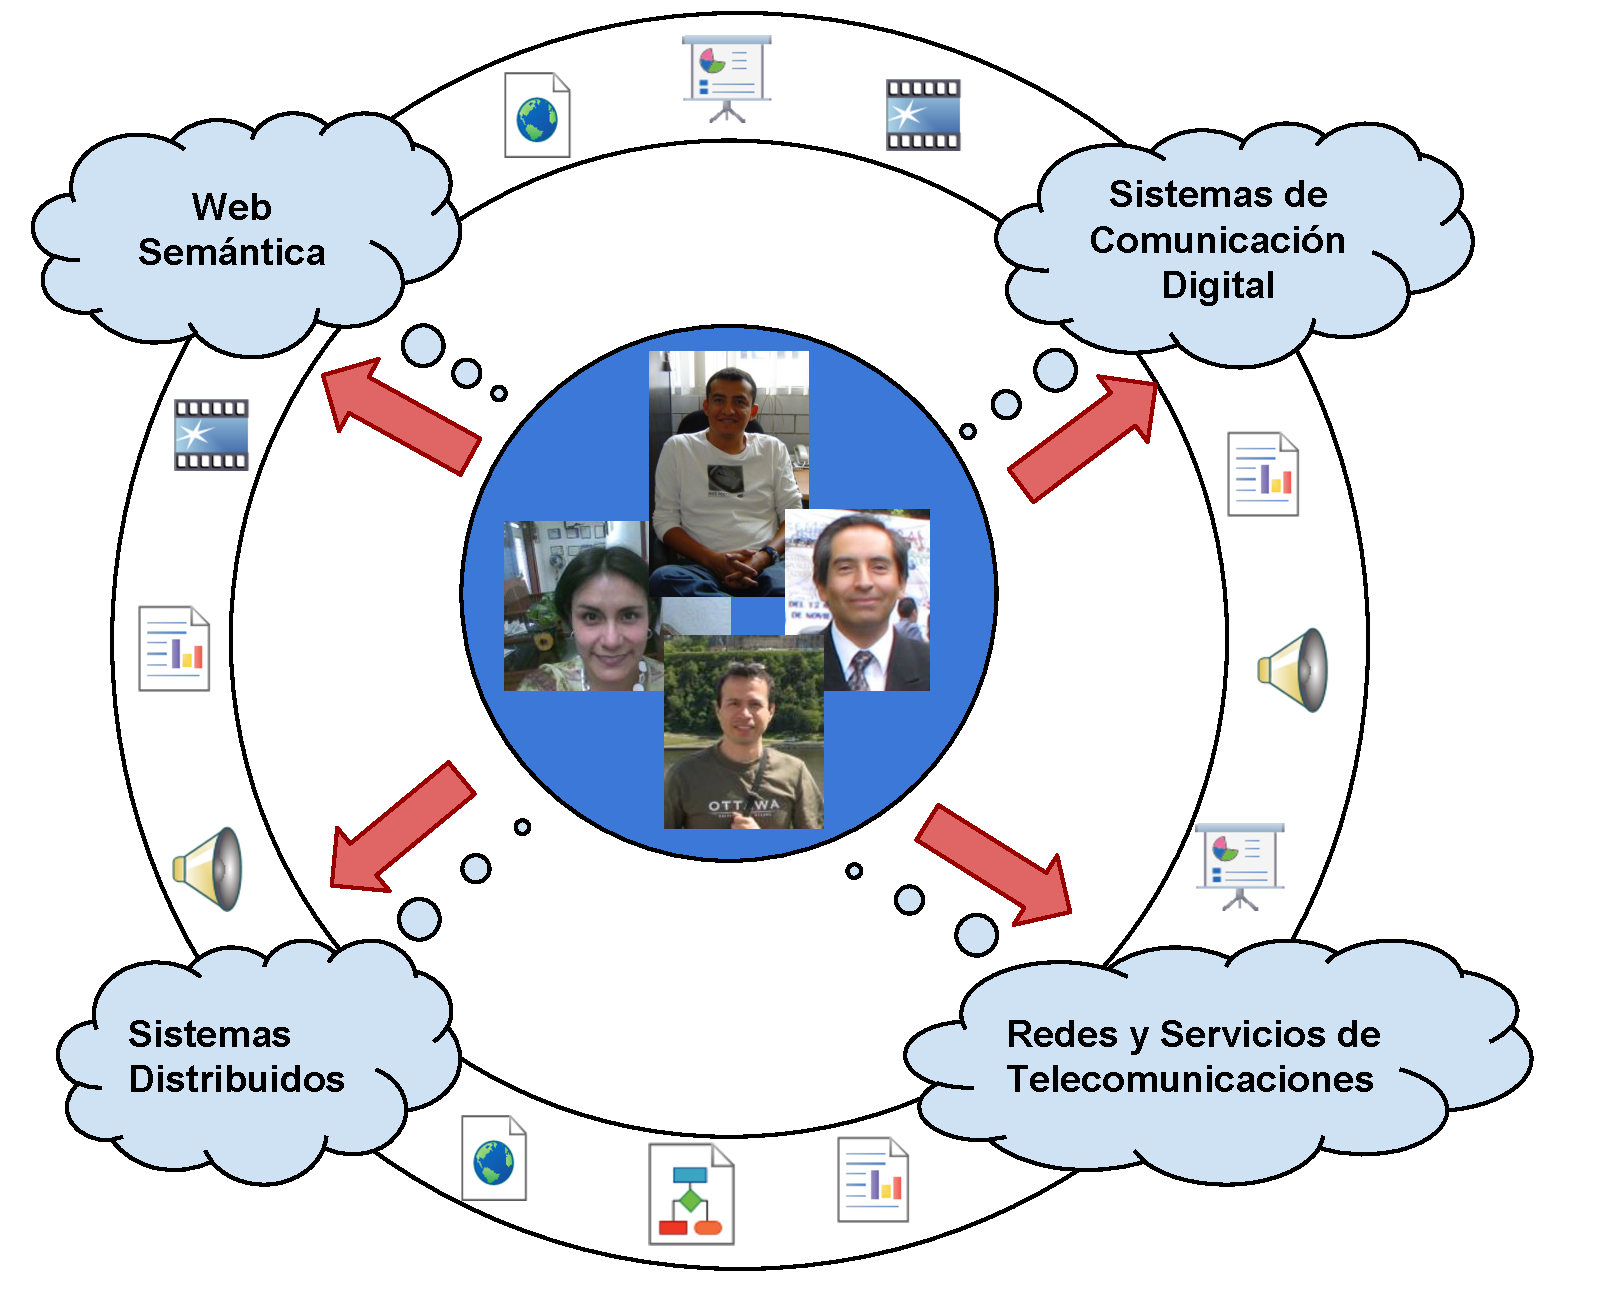
\includegraphics[scale=0.18]{ConocimientoRyT} 
	}
	\subfigure{
	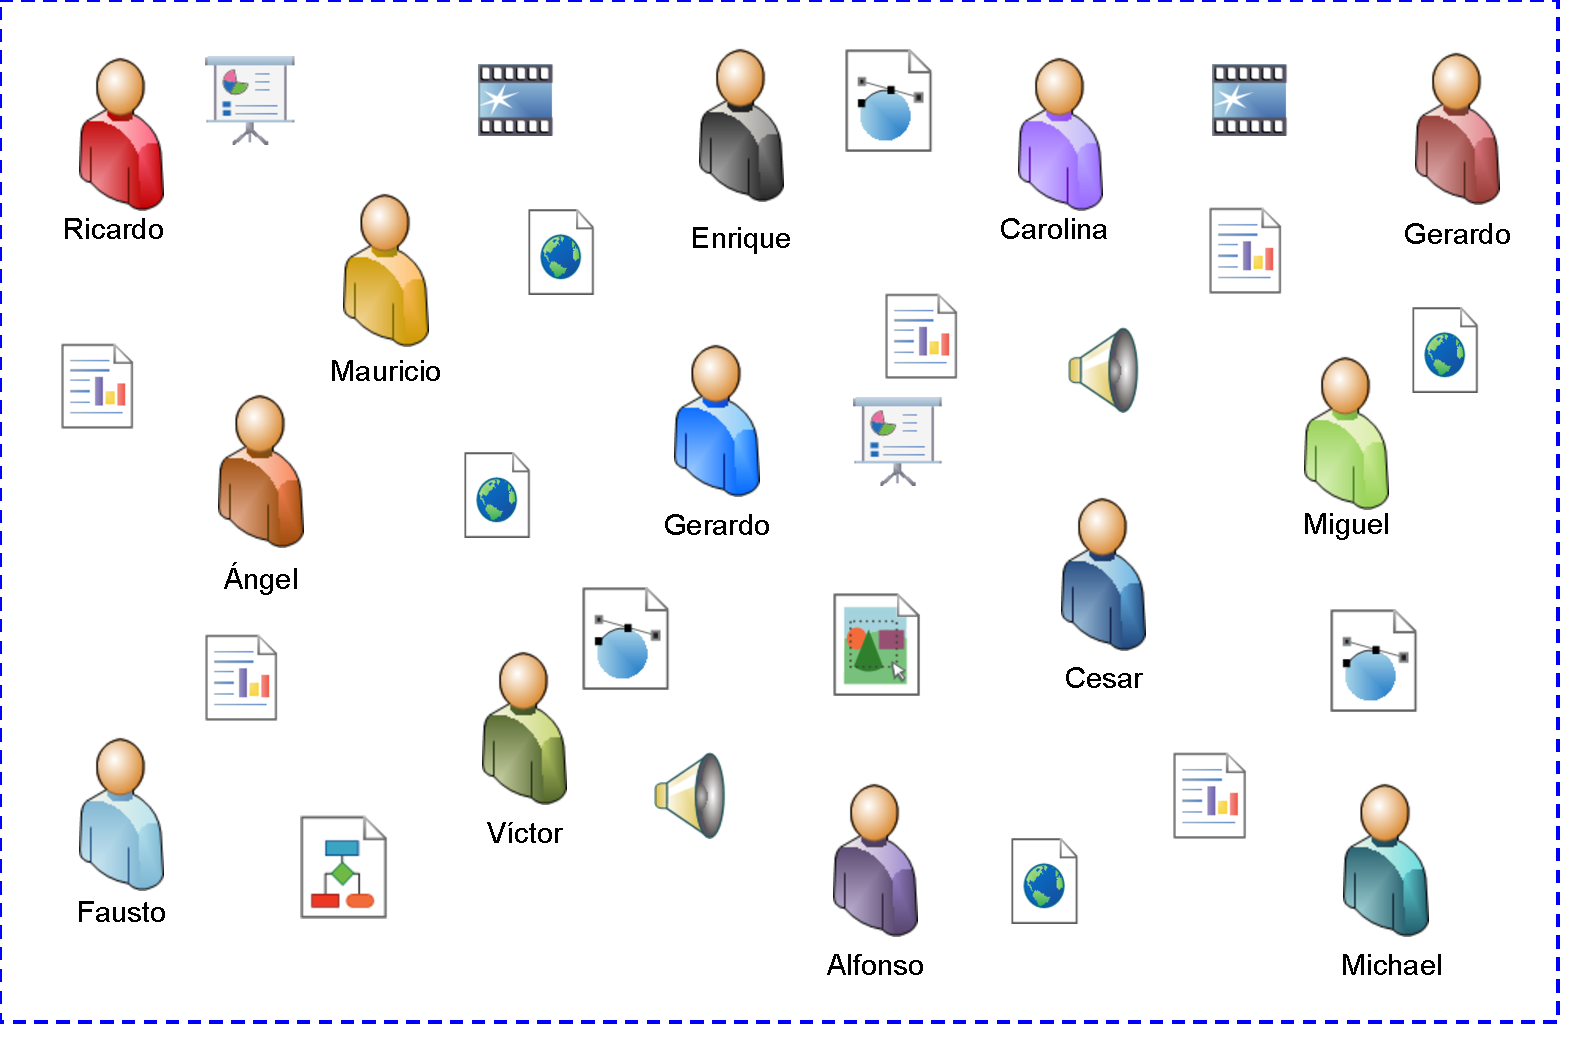
\includegraphics[scale=0.19]{EjemploMC} 
	}
	\end{figure}
	%%%%%%%%%%%%%%%%%%%%%%%
\end{frame}

\subsection{Integraci�n de la informaci�n de los recursos de informaci�n}
\begin{frame}
	\frametitle{Integraci�n de la informaci�n de los recursos de informaci�n}
	\begin{block}{Definici�n}
	\justifying
	\small La b�squeda y recuperaci�n significativa de informaci�n existente en los recursos de informaci�n para responder una consulta dada por un usuario.
	\end{block}
	
	\begin{exampleblock}{Etapas}
	\begin{enumerate}[<+-| alert@+>]
	\item \justifying \small Representar el conocimiento e informaci�n de los \textit{recursos de informaci�n}.
	\item \justifying \small Buscar y recuperar informaci�n, mediante la interrogaci�n de la representaci�n de conocimiento (modelo).
	\end{enumerate}
	\end{exampleblock}
	
	\begin{figure}
	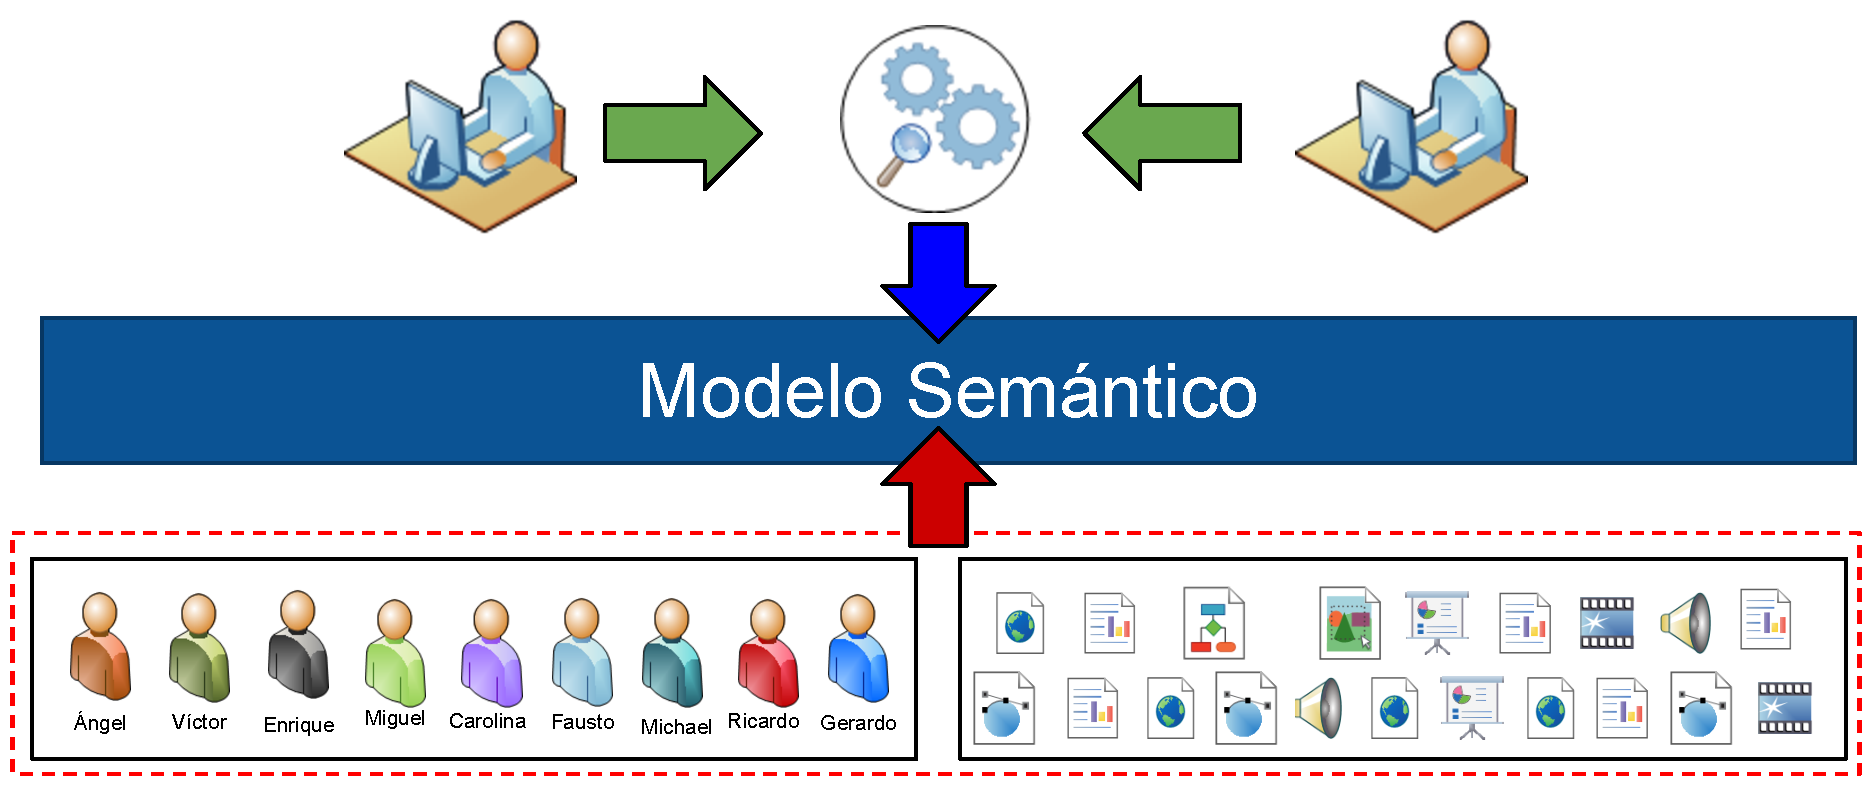
\includegraphics[scale=0.24]{IntegracionSemantica} 
	\end{figure}
\end{frame}

\subsection{Tecnolog�as Sem�nticas}
\begin{frame}
	\frametitle{Tecnolog�as Sem�nticas}
	\begin{block}{Definici�n}
	\justifying 
	\textit{Un conjunto de metodolog�as, lenguajes, aplicaciones, herramientas y est�ndares para suministrar u obtener el significado de las palabras, informaci�n y las relaciones entre �stos}. \begin{scriptsize}\cite{SemTecRetr}\end{scriptsize}
	\end{block}
	
	\begin{figure}
	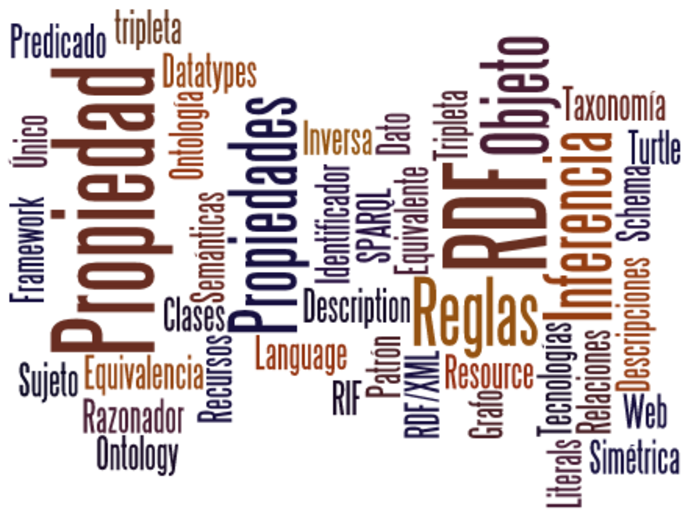
\includegraphics[scale=0.42]{TSWords} 
	\end{figure}
\end{frame}

\subsection{Integraci�n sem�ntica de recursos de informaci�n}
\begin{frame}
	\frametitle{Integraci�n sem�ntica de recursos de informaci�n}
	\begin{figure}
	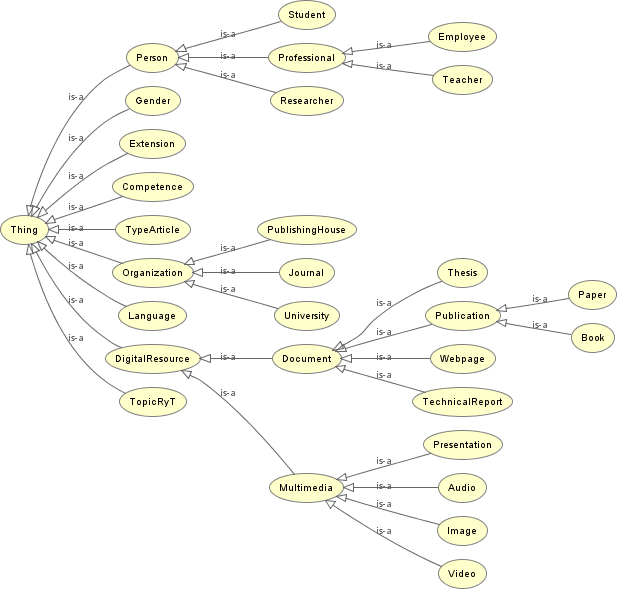
\includegraphics[scale=0.38]{ISRIMC} 
	\end{figure}
\end{frame}

\subsection{Estado del Arte}
\begin{frame}
	\frametitle{Estado del Arte}
	\begin{block}{Ejes claves}
	\begin{enumerate}
	\item \justifying Integraci�n de la informaci�n a partir del uso de tecnolog�as sem�nticas.
	\item \justifying B�squeda, recuperaci�n y publicaci�n de la informaci�n desde una ontolog�a.
	\item \justifying Gesti�n de una memoria corporativa.
	\end{enumerate}
	\end{block}
	
	\begin{figure}
	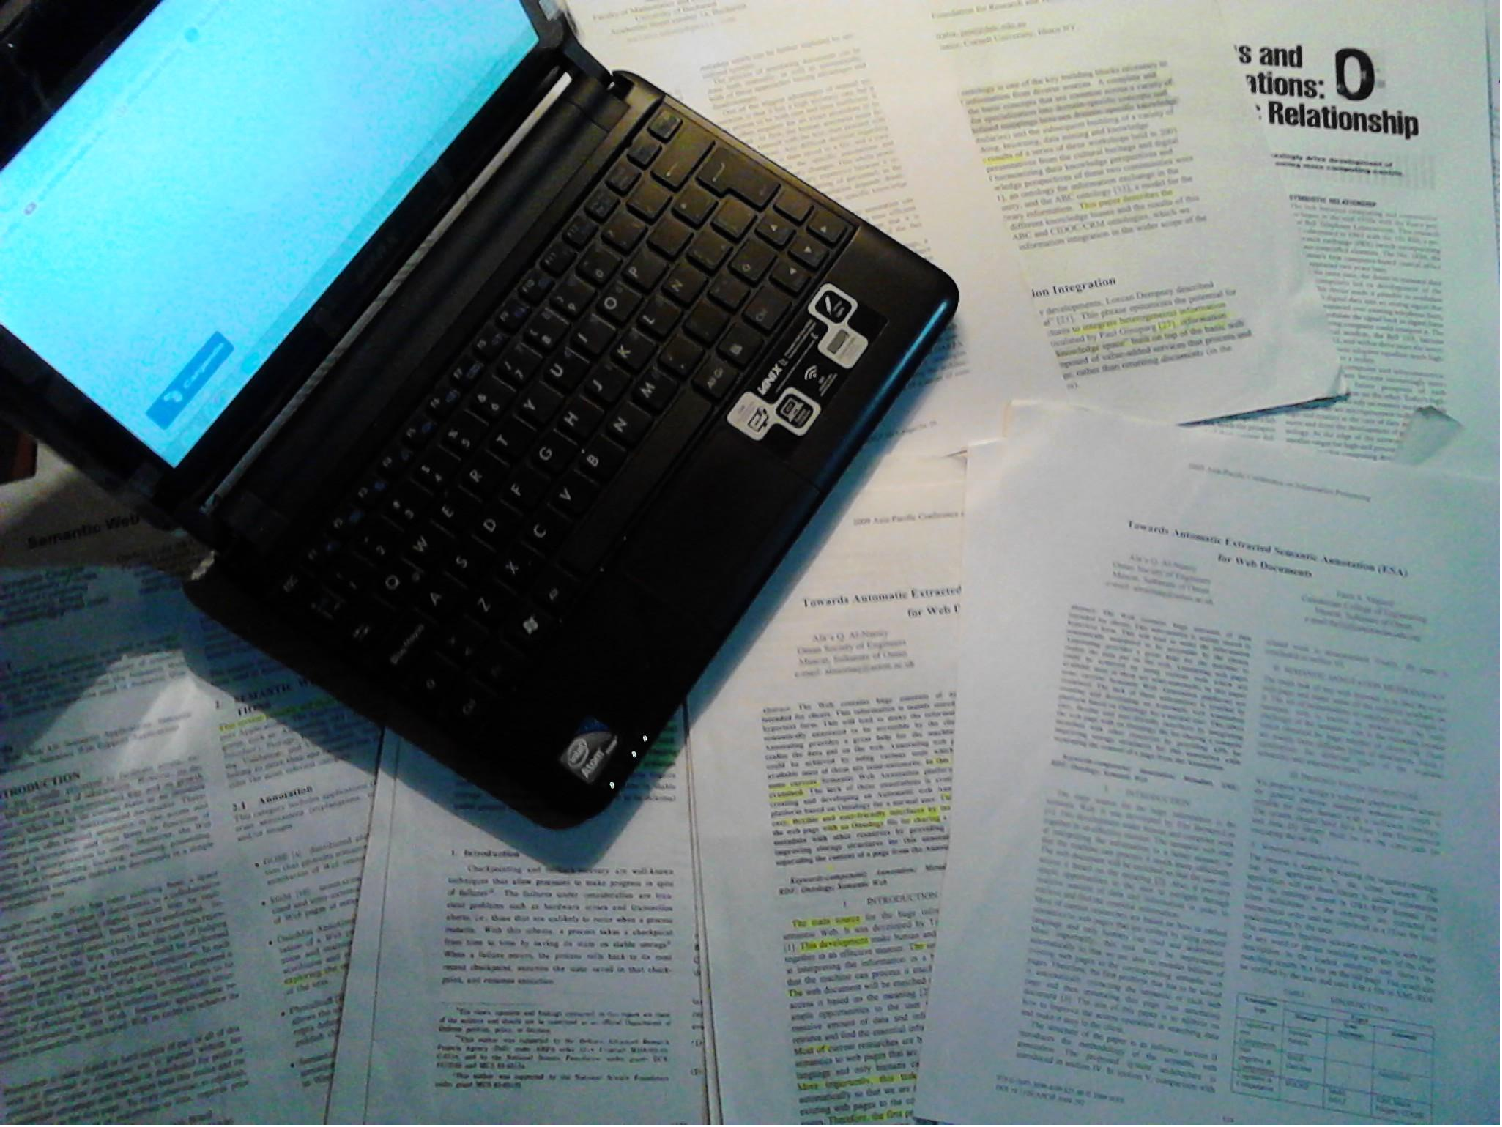
\includegraphics[scale=0.15]{EstadoArte} 
	\end{figure}
\end{frame}

\begin{frame}
	\frametitle{Comparativa}
	\begin{figure}
	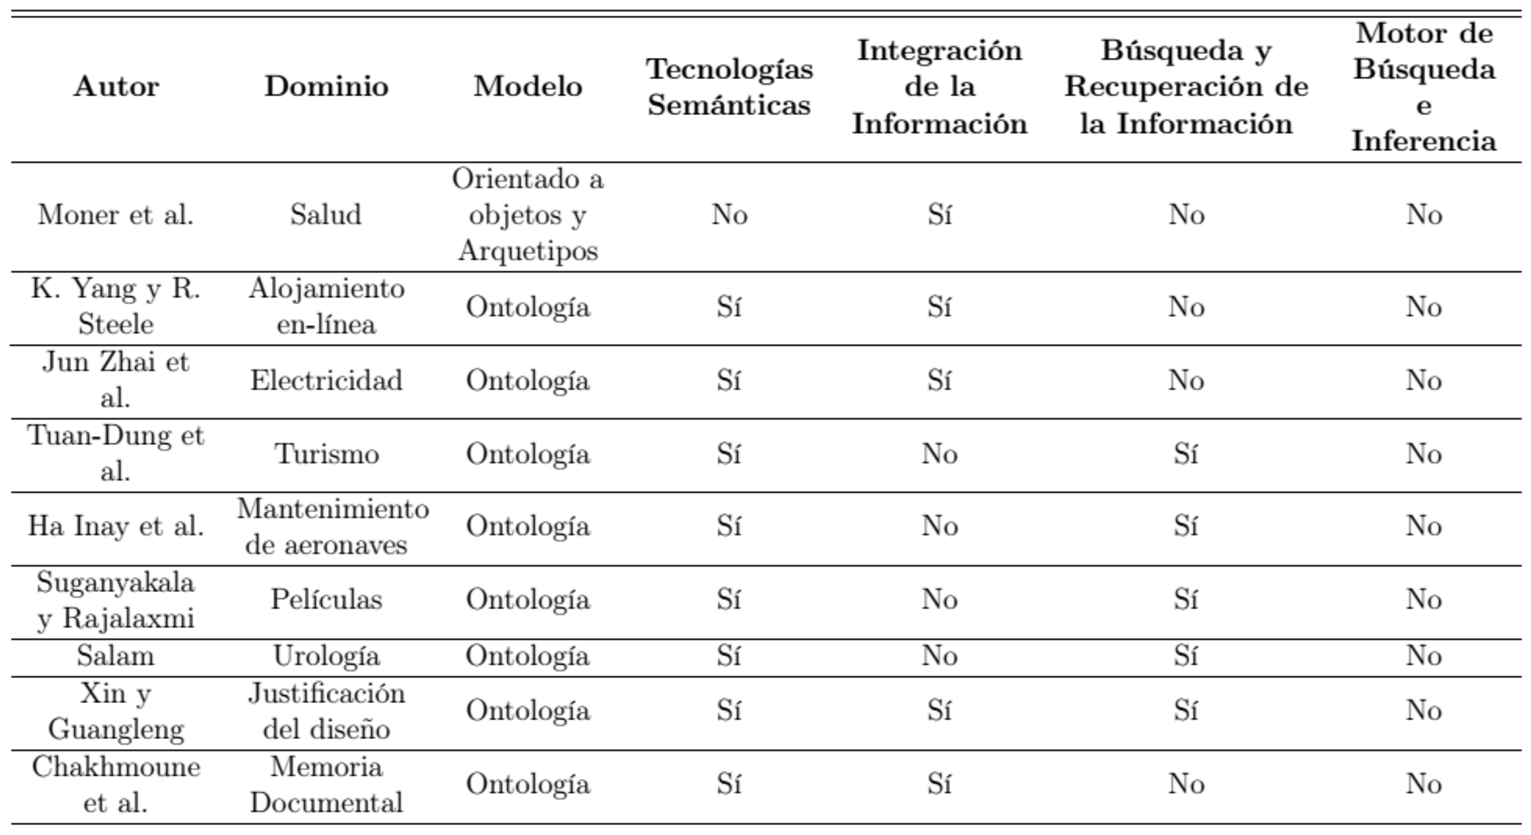
\includegraphics[scale=0.42]{TablaEOA} 
	\end{figure}
\end{frame}
\section{Descripci�n del Problema}

\subsection{Pregunta Investigaci�n}
\begin{frame}
	\frametitle{Pregunta Investigaci�n} 
	\begin{exampleblock}{}
	\justifying 
	\textit{�Las \textbf{tecnolog�as sem�nticas} son viables para solucionar la \textbf{integraci�n sem�ntica} de los \textbf{recursos de informaci�n} de una \textbf{memoria corporativa}?}
	\end{exampleblock}
	
	\begin{figure}
	
\includegraphics[scale=0.4]{PreguntaInv} 
	\end{figure}
\end{frame}

\subsection{Objetivos}
\begin{frame}
	\frametitle{Objetivos} 
	\begin{alertblock}{Objetivo Principal}
	\justifying 
	Contribuir a la \textit{integraci�n sem�ntica} de los \textit{recursos de informaci�n} en \textit{una memoria corporativa}, mediante el uso de las \textit{tecnolog�as sem�nticas}.
	\end{alertblock}
	
	\begin{block}{Objetivos Particulares}
	\begin{enumerate}
	\item \justifying \small Un \textbf{\textit{marco de referencia}} para la \textit{integraci�n sem�ntica} de los \textit{recursos de informaci�n}.
	\item \justifying \small Un \textbf{\textit{modelo sem�ntico}} que representa el \textit{conocimiento expl�cito e impl�cito} de los \textit{recursos de informaci�n}.
	\item \justifying \small Un \textbf{\textit{prototipo de interfaz gr�fica de usuario}} que permita a los usuarios consultar y visualizar la informaci�n de los recursos de informaci�n, interrogando un modelo sem�ntico.
	\item \justifying \small La evaluaci�n de la calidad de los \textbf{\textit{resultados recuperados}} y los \textbf{\textit{tiempos de procesamiento}} de la \textit{integraci�n sem�ntica}.
	\end{enumerate}
	\end{block}
\end{frame}

\subsection{Metodolog�a}
\begin{frame}
	\frametitle{Metodolog�a I}
	\begin{block}{Marco de Referencia}
	\begin{enumerate}
	\item \justifying \small Identificar los \textit{casos de uso}.
	\item \justifying \small Evaluar las \textit{herramientas sem�nticas}.
	\item \justifying \small Conformar los \textit{recurso de informaci�n} de la \textit{memoria corporativa}.
	\end{enumerate}
	
	\begin{exampleblock}{Modelo Sem�ntico}
	\begin{enumerate}
	\setcounter{enumi}{3}
	\item \justifying \small Representar el \textit{conocimiento expl�cito} de los \textit{recursos de informaci�n} en un \textit{modelo sem�ntico} (ontolog�a).
	\item \justifying \small Enriquecer el \textit{modelo sem�ntico} con \textit{reglas de inferencia}.
	\end{enumerate}
	\end{exampleblock}
	
	\begin{enumerate}
	\setcounter{enumi}{5}
	\item \justifying \small Escribir las principales \textit{consultas} en la sintaxis correspondiente.
	\item \justifying \small Emplear un razonador para hacer expl�cito el conocimiento impl�cito.
	\item \justifying \small Buscar y recuperar informaci�n en la memoria corporativa, interrogando el modelo sem�ntico inferido.
	\end{enumerate}
	\end{block}
\end{frame}

\begin{frame}
	\frametitle{Metodolog�a II}	
	\begin{block}{Prototipo de interfaz gr�fica de usuario}	
	\begin{enumerate}
	\setcounter{enumi}{8}
	\item \justifying \small Construir el \textit{prototipo de interfaz de usuario} para la (b�squeda y navegaci�n) de los usuarios en un modelo sem�ntico.
	\end{enumerate}
	\end{block}
	
	\begin{block}{Evaluaci�n}
	\begin{enumerate}
	\setcounter{enumi}{9}
	\item \justifying \small Evaluar la calidad de los resultados con y sin inferencia.
	\item \justifying \small Evaluar los \textit{tiempos promedios} de consulta sobre modelos con/sin inferencia.
	\end{enumerate}
	\end{block}
\end{frame}

\subsection{Hip�tesis}
\begin{frame}
	\frametitle{Hip�tesis}
	\begin{block}{}
	\justifying 
	\textbf{El uso de las \textit{tecnolog�as sem�nticas} es adecuado para lograr la \textit{integraci�n sem�ntica} de \textit{recursos de informaci�n} en una \textit{memoria corporativa}}.
	\end{block}
	
	\begin{figure}
	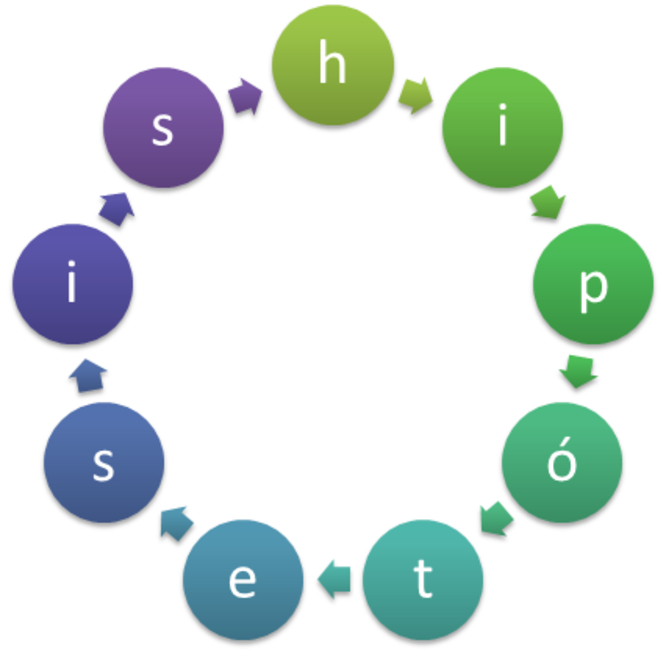
\includegraphics[scale=0.45]{hipotesis} 
	\end{figure}
\end{frame}

\subsection{Aportaciones}
\begin{frame}
	\frametitle{Aportaciones}
	\begin{enumerate}
	\item \justifying Un \textit{marco de referencia} para lograr la \textit{integraci�n sem�ntica} de \textit{recursos de informaci�n}.
    \item \justifying Un modelo sem�ntico que representa el conocimiento de una memoria corporativa.
    \item \justifying  Un prototipo (interfaz gr�fica de usuario) para la interacci�n amigable (b�squeda y consulta de informaci�n) de los usuarios con el modelo sem�ntico.
    \item \justifying Los resultados de nuestra evaluaci�n experimental.
    \item \justifying Un par de scripts para la generaci�n autom�tica y controlada de descripciones (conocimiento expl�cito) de los \textit{recursos de informaci�n}.
	\end{enumerate}
\end{frame}
%%%%%%%%%%%%%%%%%%%%%%%%%%%%%%%%%%%%%%%%%%%%%%%%%%%%%%%%%%%%%%%%%%%%%%%%%%%%%%
\section{Integraci�n Sem�ntica de una Memoria Corporativa}
%%%%%%%%%%%%%%%%%%%%%%%%%%%%%%%%%%%%%%%%%%%%%%%%%%%%%%%%%%%%%%%%%%%%%%%%%%%%%%
\begin{frame}
	\frametitle{Marco de Referencia}
	\begin{block}{Etapas}
		\begin{enumerate}
		\item \justifying Representar las caracter�sticas y/o relaciones de los \textit{recursos de informaci�n} mediante el est�ndar RDF, para construir un modelo sem�ntico.
		\item \justifying Introducir \textit{reglas de inferencia} en el modelo sem�ntico, para enriquecer con \textit{conocimiento impl�cito} de los \textit{recursos de informaci�n} y del dominio de la memoria.
		\item \justifying Buscar y recuperar informaci�n en el modelo sem�ntico para responder un conjunto consultas SPARQL.
		\end{enumerate}
	\end{block}
\end{frame}
%%%%%%%%%%%%%%%%%%%%%%%%%%%%%%%%%%%%%%%%%%%%%%%%%%%%%%%%%%%%%%%%%%%%%%%%%%%%%%

%%%%%%%%%%%%%%%%%%%%%%%%%%%%%%%%%%%%%%%%%%%%%%%%%%%%%%%%%%%%%%%%%%%%%%%%%%%%%%
\begin{frame}
	\frametitle{Arquitectura de la Integraci�n Sem�ntica}	
	\begin{figure}
	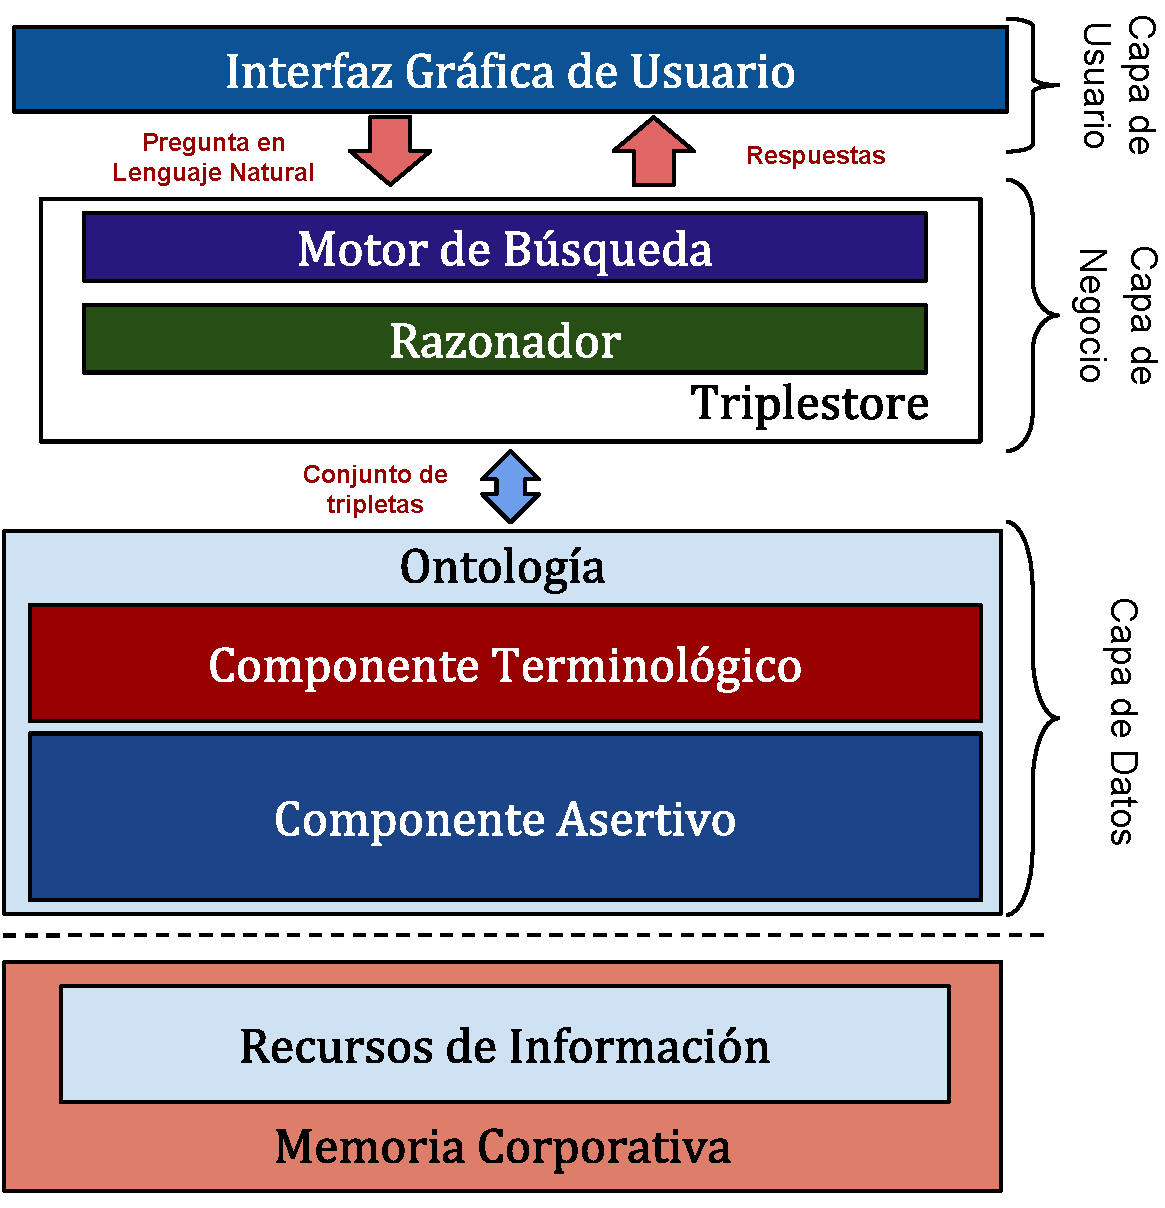
\includegraphics[scale=0.33]{Arquitectura} 
	\end{figure}
\end{frame}
%%%%%%%%%%%%%%%%%%%%%%%%%%%%%%%%%%%%%%%%%%%%%%%%%%%%%%%%%%%%%%%%%%%%%%%%%%%%%%

%%%%%%%%%%%%%%%%%%%%%%%%%%%%%%%%%%%%%%%%%%%%%%%%%%%%%%%%%%%%%%%%%%%%%%%%%%%%%%
\begin{frame}
	\frametitle{Casos de Uso}
	
	\begin{block}{}
		\begin{itemize}
		\item \justifying \textbf{\textit{Cartograf�a de Competencias}} es la b�squeda y recuperaci�n de informaci�n significativa de las personas a partir de las caracter�sticas personales y profesionales de las mismas.
		\item \justifying \textbf{\textit{B�squeda de Recursos Digitales}} es la b�squeda y recuperaci�n de informaci�n significativa de los documentos y archivos multimedia a partir del contenido de los mismos.
		\end{itemize}
	\end{block}
	
	\begin{figure}
	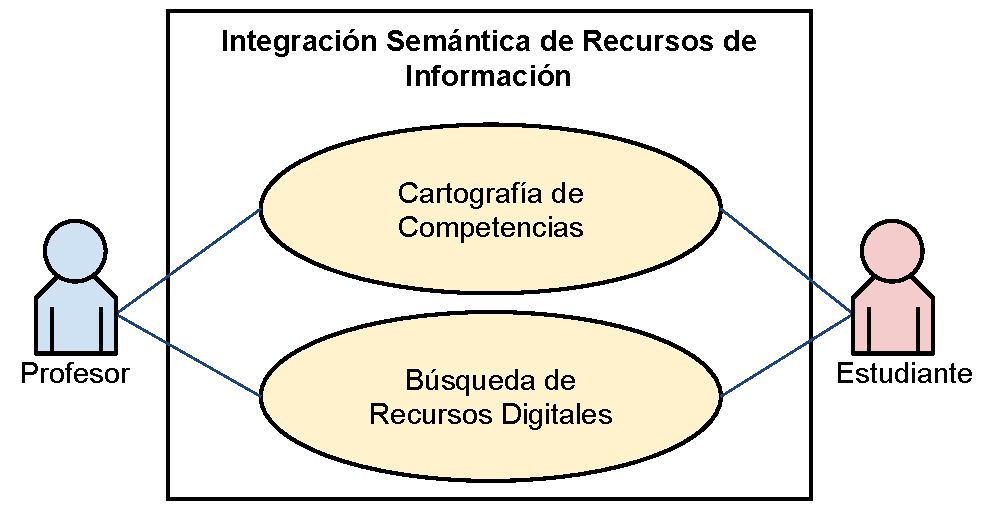
\includegraphics[scale=0.56]{CasosUso} 
	\end{figure}
\end{frame}
%%%%%%%%%%%%%%%%%%%%%%%%%%%%%%%%%%%%%%%%%%%%%%%%%%%%%%%%%%%%%%%%%%%%%%%%%%%%%%

%%%%%%%%%%%%%%%%%%%%%%%%%%%%%%%%%%%%%%%%%%%%%%%%%%%%%%%%%%%%%%%%%%%%%%%%%%%%%%
\subsection{Representaci�n el Conocimiento}
\subsubsection{Identificar los principales recursos de informaci�n}
\begin{frame}
	\frametitle{Identificar los principales recursos de informaci�n}	
	\begin{figure}
	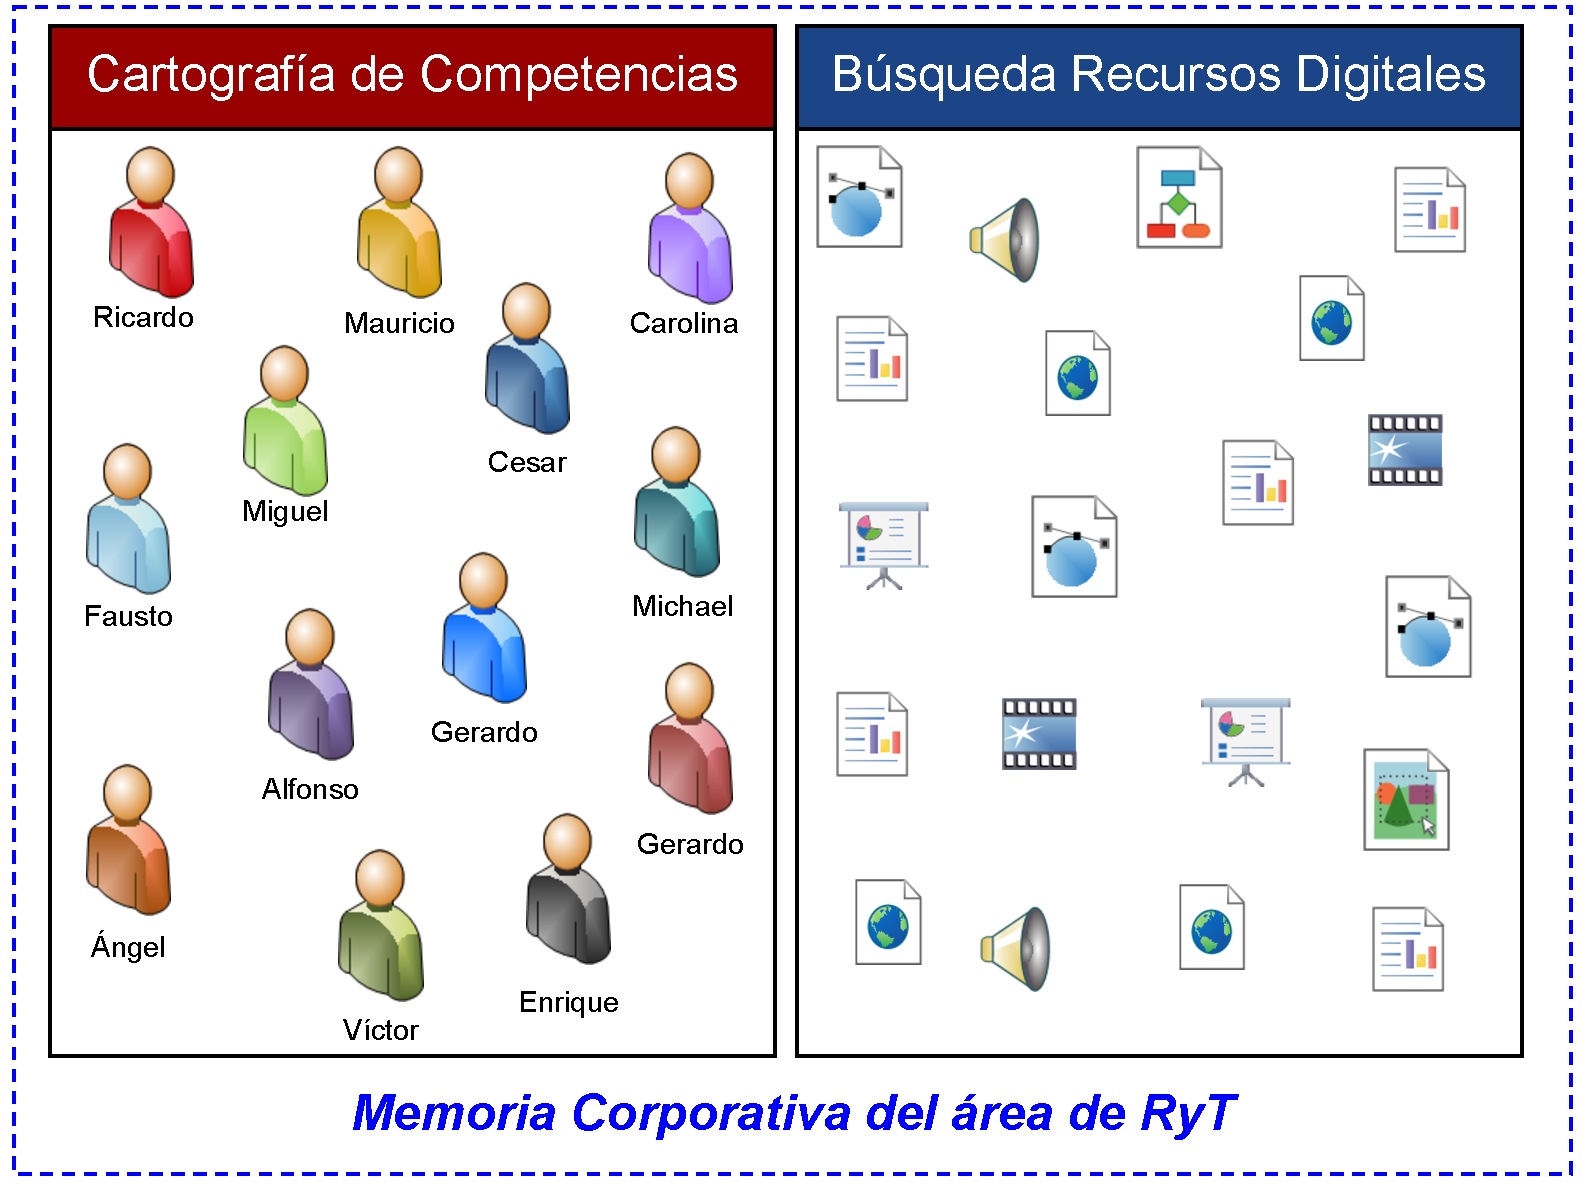
\includegraphics[scale=0.33]{CasosUsoMC} 
	\end{figure}
\end{frame}

\subsubsection{Adquirir y expresar el conocimiento de los recursos de informaci�n}
\begin{frame}
	\frametitle{Adquirir y expresar el conocimiento de los recursos de informaci�n}	
	\begin{figure}
	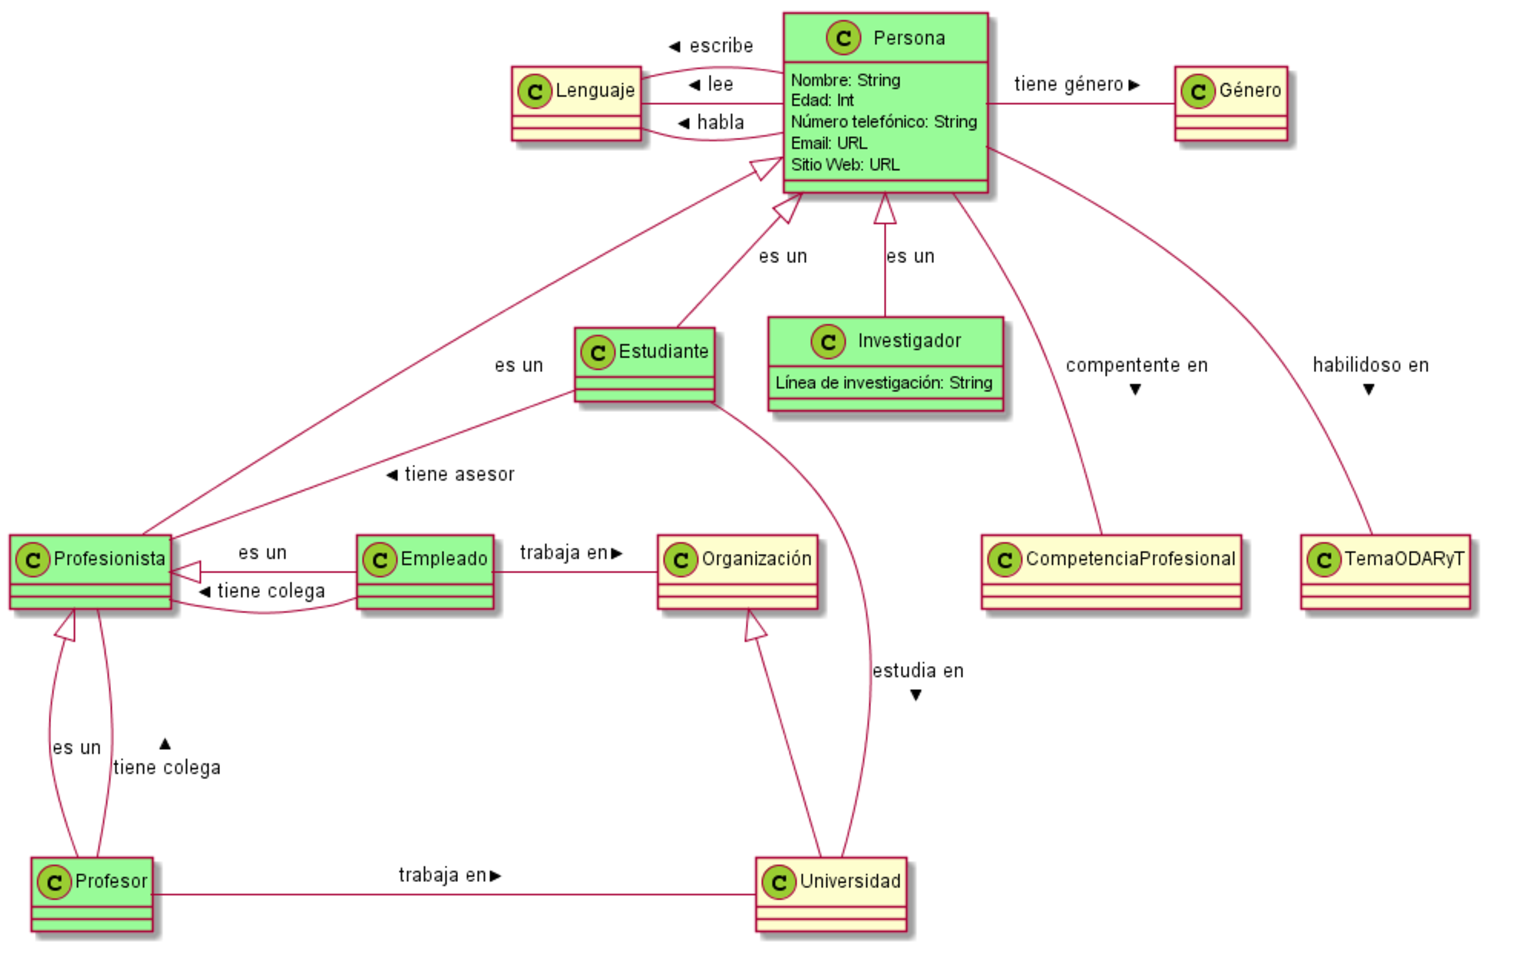
\includegraphics[scale=0.38]{CasoUsoCartComp} 
	\end{figure}
\end{frame}

\subsubsection{Representar el conocimiento e informaci�n mediante el est�ndar RDF}
\begin{frame}
	\frametitle{Representar el conocimiento e informaci�n mediante el est�ndar RDF}
	
	\begin{block}{Definici�n}
	\justifying 
	Marco gen�rico para describir el conocimiento e informaci�n expl�cita de los recursos mediante sus caracter�sticas y relaciones. \begin{scriptsize}\cite{SurvSemWeb2012}\end{scriptsize}
	\end{block}
	
	\begin{block}{Actividades en la representaci�n del conocimiento}
	\begin{enumerate}
	\item \justifying Asignar un \textit{identificador �nico de recursos} (URI) a cada \textit{recurso de informaci�n} en la \textit{memoria corporativa}.
	\item \justifying Asignar un URI a cada caracter�stica y/o relaci�n (propiedad) de de los \textit{recursos de informaci�n}.
	\item \justifying Generar las tripletas RDF asociadas a las descripciones de los recursos de informaci�n.
	\end{enumerate}
	\end{block}
%	\begin{figure}
%	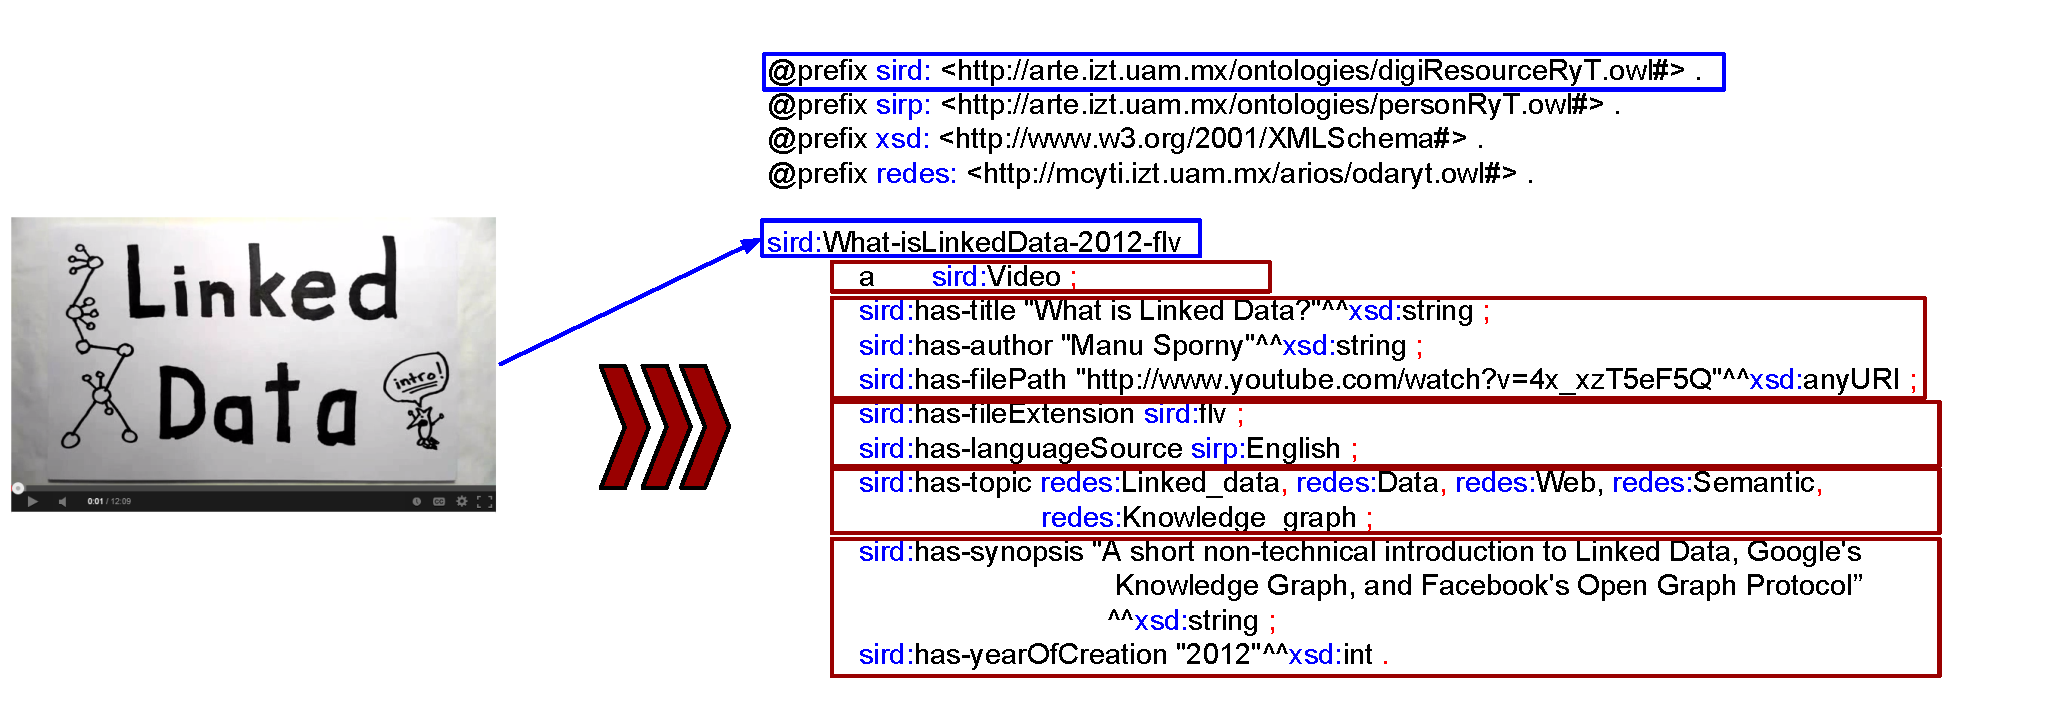
\includegraphics[scale=0.38]{Vid2RDF}
%	\end{figure}
	%%%%%%%%%%%%%%%%%%%%%%%
\end{frame}

\begin{frame}
	\frametitle{Representar el conocimiento e informaci�n mediante el est�ndar RDF}
	\begin{figure}
	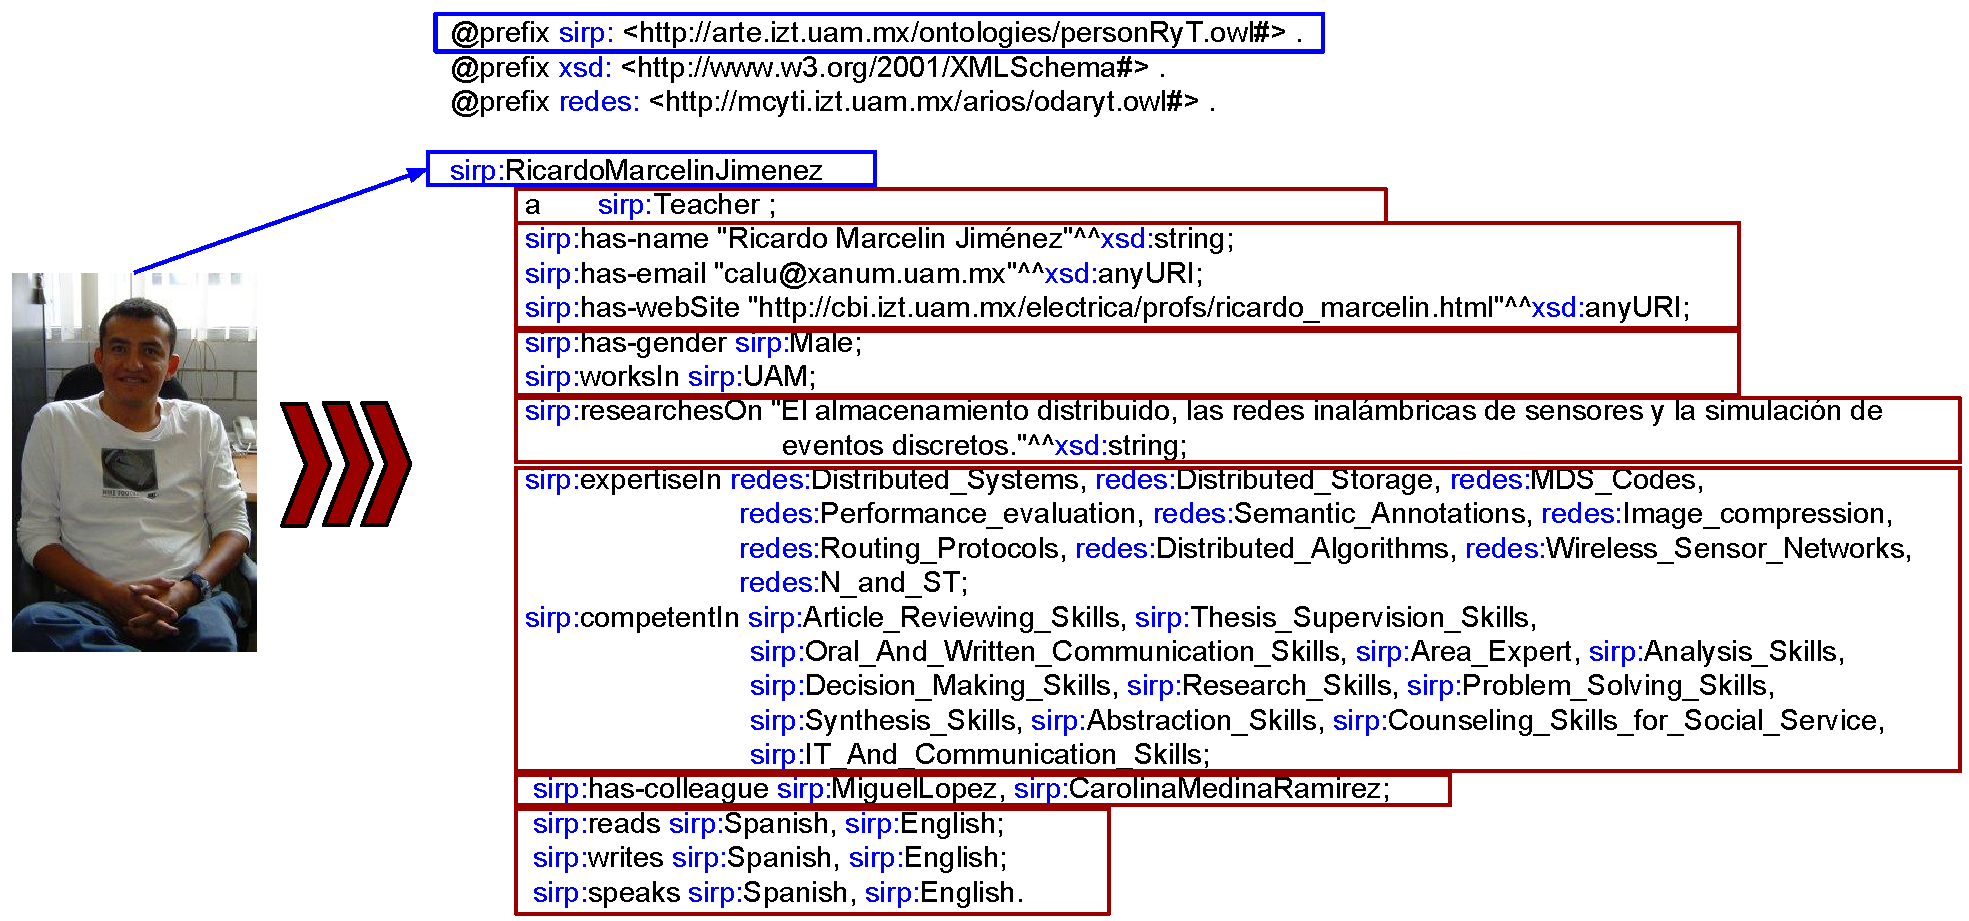
\includegraphics[scale=0.35]{Person2RDF}
	\end{figure}
\end{frame} 

\begin{frame}
	\frametitle{Representar el conocimiento e informaci�n mediante el est�ndar RDF}
	\begin{figure}
	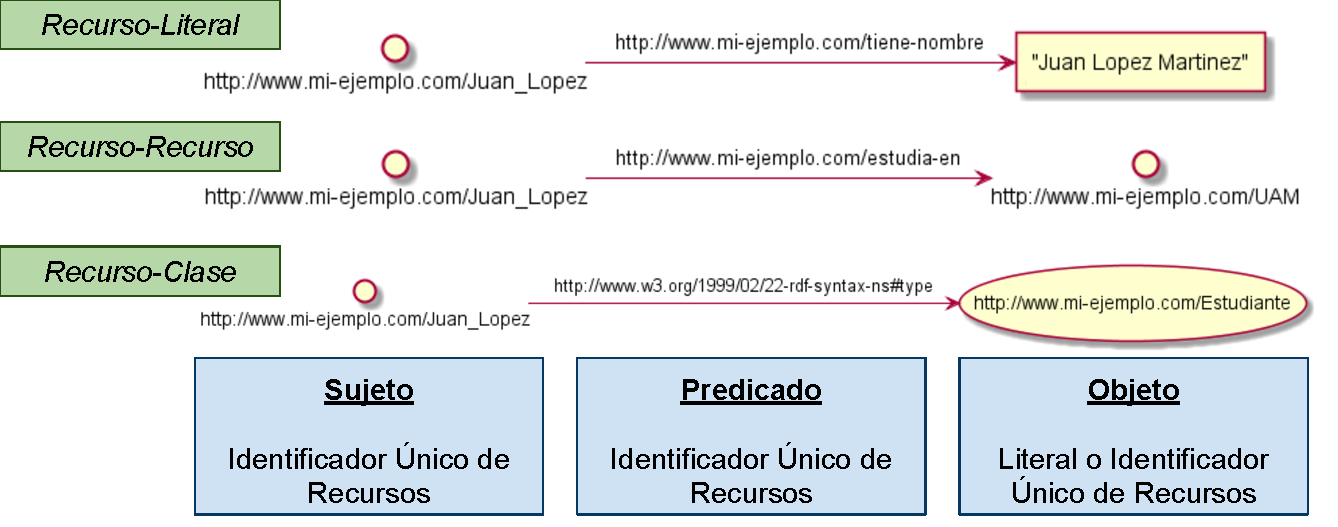
\includegraphics[scale=0.45]{Tripletas} 
	\end{figure}
\end{frame}

\begin{frame}
	\frametitle{Representar el conocimiento e informaci�n mediante el est�ndar RDF}
	\begin{figure}
	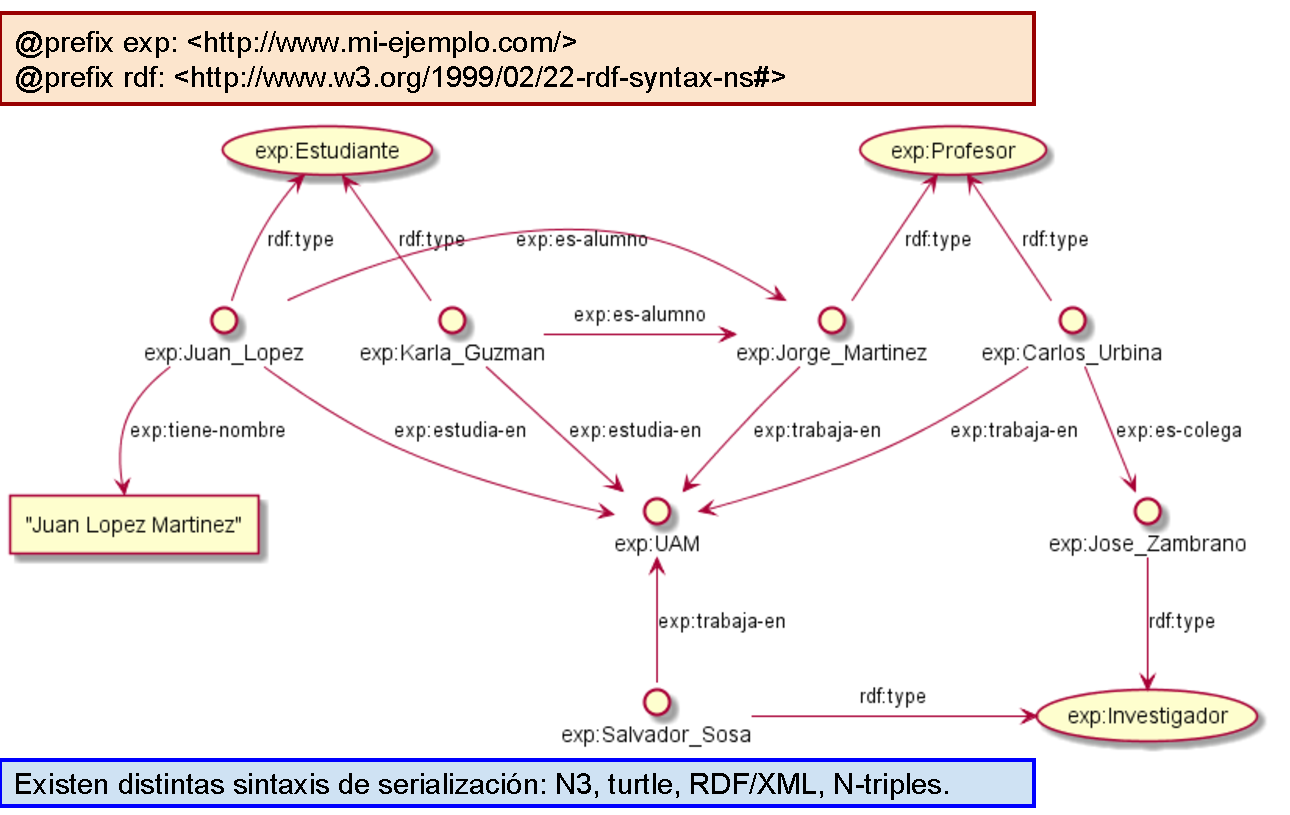
\includegraphics[scale=0.48]{GrafoRDF} 
	\end{figure}
\end{frame}

%%%%%%%%%%%%%%%%%%%%%%%%%%%%%%%%%%%%%%%%%%%%%%%%%%%%%%%%%%%%%%%%%%%%%%%%%%%%%%

\subsection{Enriquecer el conocimiento en el modelo sem�ntico}
\begin{frame}
	\frametitle{Ontolog�a}
	%%%%%%%%%%%%%%%%%%%%%%%%%%%%
	\begin{alertblock}{Definici�n}
	\justifying 
	Una definici�n formal, expl�cita y compartida de los conceptos, as� como las relaciones de un determinado dominio. \begin{scriptsize}\cite{Gruber}\end{scriptsize}
	\end{alertblock}
	
	\begin{block}{Componentes}
	\begin{itemize}
	\item \justifying \textbf{\textit{Componente Asertivo (ABox)}} est� constituido por descripciones que afirman que los individuos son instancias de una clase o propiedad.
	\item \justifying \textbf{\textit{Componente Terminol�gico (TBox)}} describe las clases y propiedades relevantes, as� como las reglas de inferencia que permiten aprovechar la manera en que las instancias se relacionan entre s�.
	\end{itemize}
	\end{block}
	%%%%%%%%%%%%%%%%%%%%%%%%%%%%
\end{frame}

\begin{frame}
	\frametitle{Axiomatizaci�n}	
	\begin{block}{Reglas de inferencia o Axiomas}
	\justifying 
	Expresiones para enriquecer un grafo RDF con conocimiento impl�cito.\\
	\end{block}
	
	\begin{block}{Lenguajes}
	Especificaciones para describir clases, propiedades e individuos.
	\begin{itemize}
	\item \justifying \textit{RDF Schema \textbf{RDF(S)}}
	\item \justifying \textit{Web Ontology Language \textbf{OWL}} 
	\end{itemize}
	\end{block}
	
	\begin{figure}
	
\includegraphics[scale=0.4]{PrefijosRDFSOWL}
	\end{figure}
	
	\begin{block}
	\justifying
	\textit{Lo que es obvio para un humano, no lo es para una maquina}.
	\end{block}
\end{frame}

%\begin{frame}
%	\frametitle{Enriquecer el conocimiento en el modelo sem�ntico}
%	\begin{block}{}
%	\justifying
%	Para cada \textit{caso de uso} debe encontrarse el respectivo conjunto de axiomas (TBox).
%	\end{block}
%	
%	\begin{figure}
%	
\includegraphics[scale=0.4]{PrefijosRDFSOWL}
%	\end{figure}
%\end{frame}
	
\subsubsection{Herencia de Clases}
\begin{frame}[allowframebreaks]
	\frametitle{Herencia de Clases}
	\begin{block}{Subclase (rdfs:subClassOf)}
	\justifying
	Afirma que una \textit{clase A} se subsume por una \textit{clase B}, es decir, la clase A es un caso particular de la \textit{clase B}. En este caso, las instancias de la clase A son instancias de la clase B.
	\end{block}
	
	\begin{figure}
	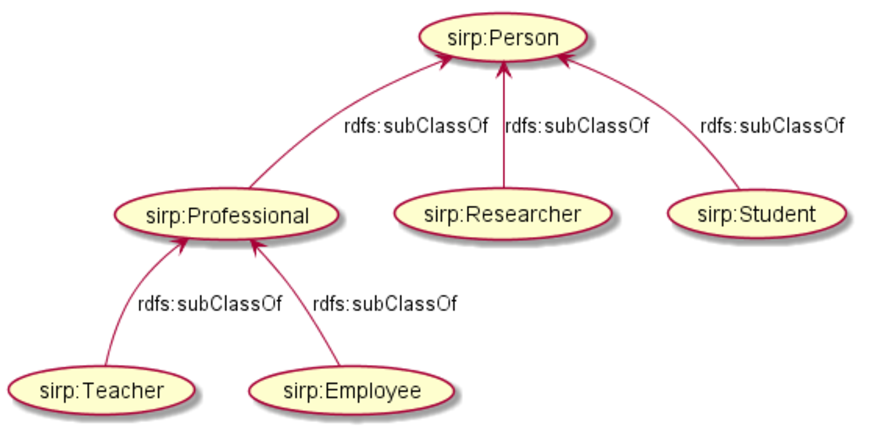
\includegraphics[scale=0.5]{HerenClassCartComp}
	\end{figure}
	%%%%%%%%%%%%%%%%%%%%%%%
	
	\begin{figure}
	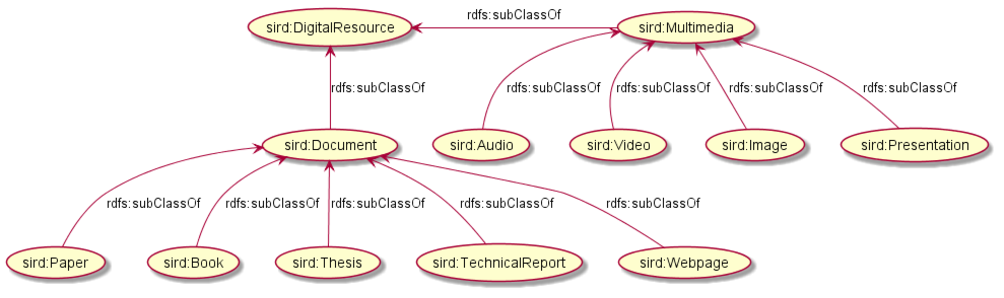
\includegraphics[scale=0.68]{HerenClassRecDigi}
	\end{figure}
	%%%%%%%%%%%%%%%%%%%%%%%
	
	\begin{figure}
	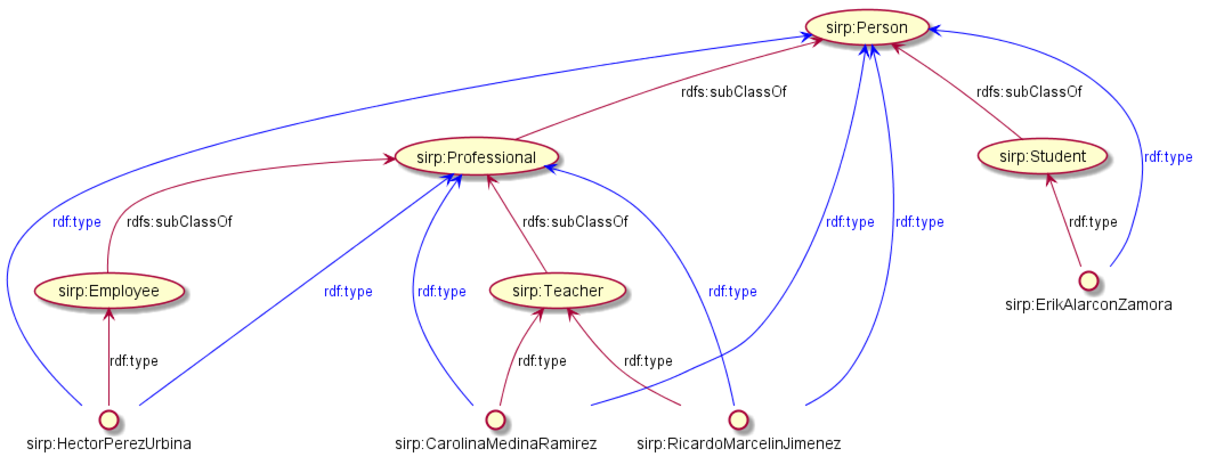
\includegraphics[scale=0.57]{EjmpInfSubClass}
	\end{figure}
	%%%%%%%%%%%%%%%%%%%%%%%
\end{frame}

\subsubsection{Herencia de Propiedades}
\begin{frame}[allowframebreaks]
	\frametitle{Herencia de Propiedades}
	\begin{block}{Subpropiedad (rdfs:subPropertyOf)}
	\justifying
	Afirma que todos los recursos que se relacionan por la \textit{propiedad X}, tambi�n se relacionan por la \textit{propiedad Y}.
	\end{block}
	
	\begin{figure}
	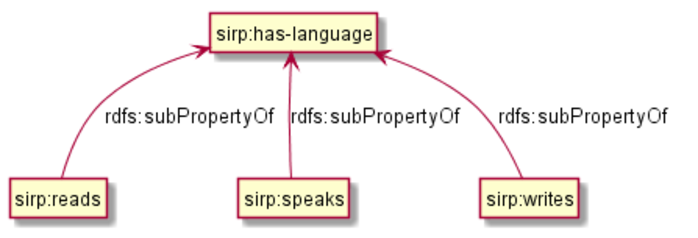
\includegraphics[scale=0.57]{HerPropLang}
	\end{figure}
		
	\begin{figure}
	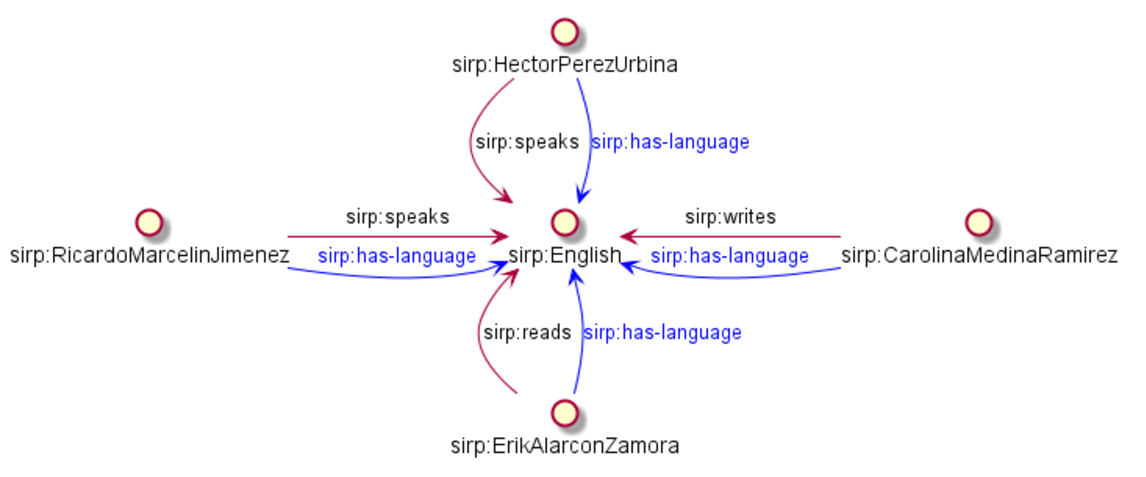
\includegraphics[scale=0.55]{EjmpInfProp}
	\end{figure}
	%%%%%%%%%%%%%%%%%%%%%%%
\end{frame}

\subsubsection{Dominio y Rango en las Propiedades}
\begin{frame}[allowframebreaks]
	\frametitle{Dominio y Rango en las Propiedades}
	\begin{block}{Dominio (rdfs:domain)}
	\justifying
	Especifica qu� clase se aplica a una propiedad.
	\end{block}
	
	\begin{block}{Rango (rdfs:range)}
	\justifying
	Especifica los valores (clase o tipo de literal) que puede asumir una propiedad.
	\end{block}
	
	\begin{figure}
	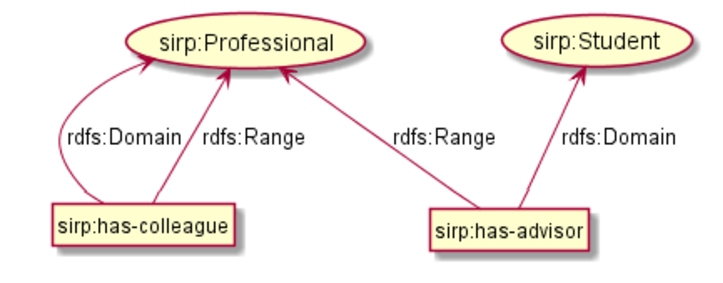
\includegraphics[scale=0.52]{exAxDyRPer}
	\end{figure}
	%%%%%%%%%%%%%%%%%%%%%%%
	
	\begin{figure}
	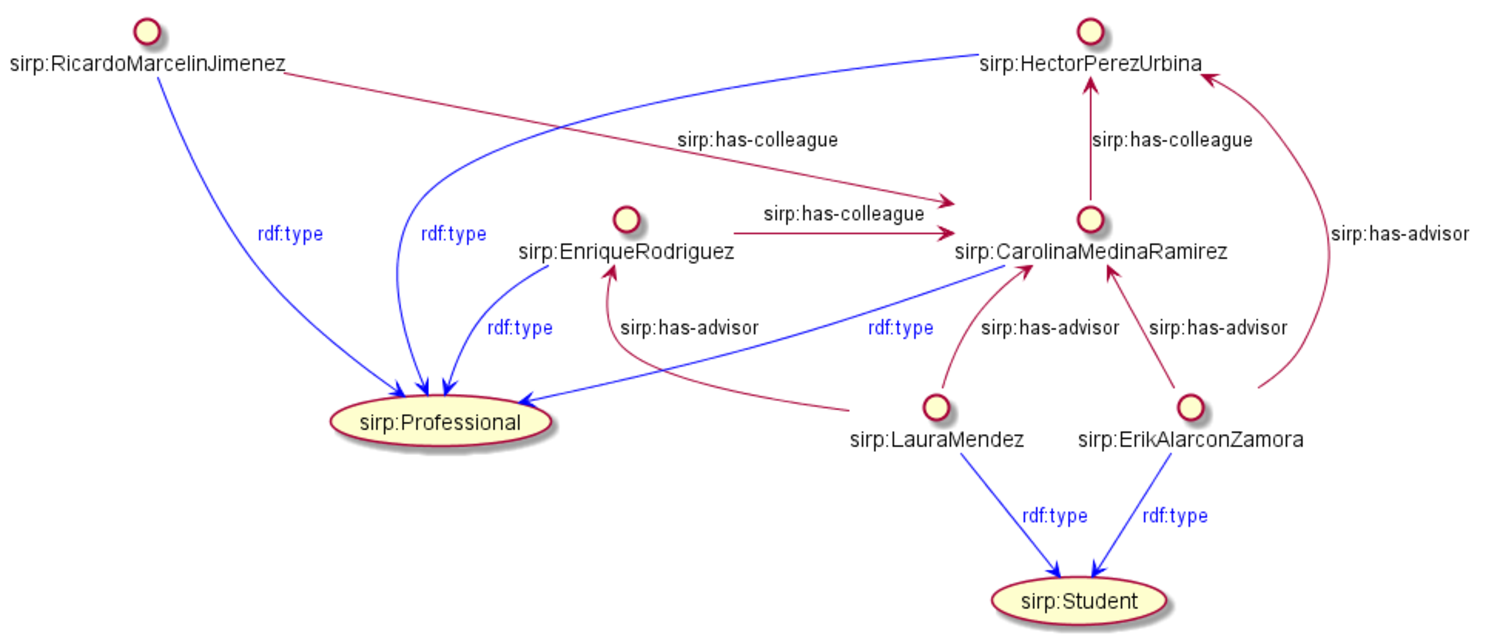
\includegraphics[scale=0.45]{exInfDyRPer}
	\end{figure}
	%%%%%%%%%%%%%%%%%%%%%%%
\end{frame}

\subsubsection{Caracter�sticas en las Propiedades}
\begin{frame}
	\frametitle{Caracter�sticas en las propiedades}
	\begin{block}{Propiedad sim�trica (owl:SymmetricProperty)}
	\justifying
	Afirma que la \textit{propiedad X} es su propia propiedad inversa, es decir, si la \textit{propiedad X} relaciona al \textit{individuo A} con el \textit{individuo B}, entonces, esta propiedad debe relacionar al \textit{individuo B} con el \textit{individuo A}.
	\end{block}
	
	\begin{figure}
	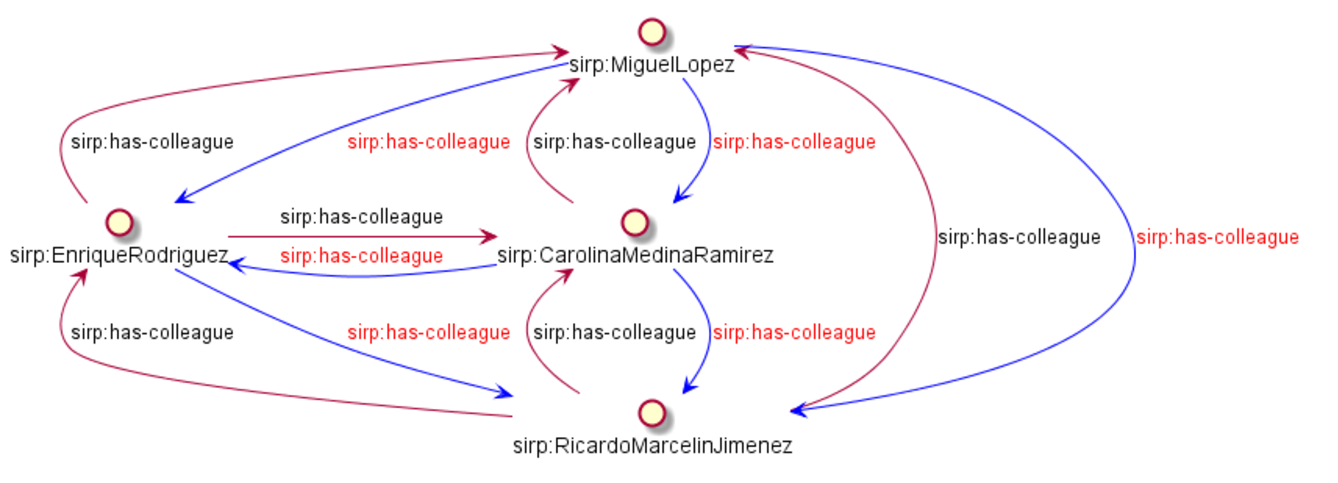
\includegraphics[scale=0.5]{infSymColl}
	\end{figure}
	%%%%%%%%%%%%%%%%%%%%%%%
\end{frame}
%%%%%%%%%%%%%%%%%%%%%%%%%%%%%%%%%%%%%%%%%%%%%%%%%%%%%%%%%%%%%%%%%%%%%%%%%%%%%%

\subsection{Buscar y recuperar la informaci�n en el modelo sem�ntico}
\begin{frame}
	\frametitle{Buscar y recuperar la informaci�n en el modelo sem�ntico}
%	\begin{block}{Objetivo}
%	\justifying
%	La b�squeda y recuperaci�n de la informaci�n para responder las preguntas o necesidades informativas de los usuarios del �rea de Redes y Telecomunicaciones (RyT).
%	\end{block}
	
	\begin{block}{SPARQL}
	\justifying 
	Lenguaje de consulta y protocolo de acceso a RDF, para la b�squeda y recuperaci�n de la informaci�n en un grafo RDF.
	\end{block}
	
	\begin{figure}
	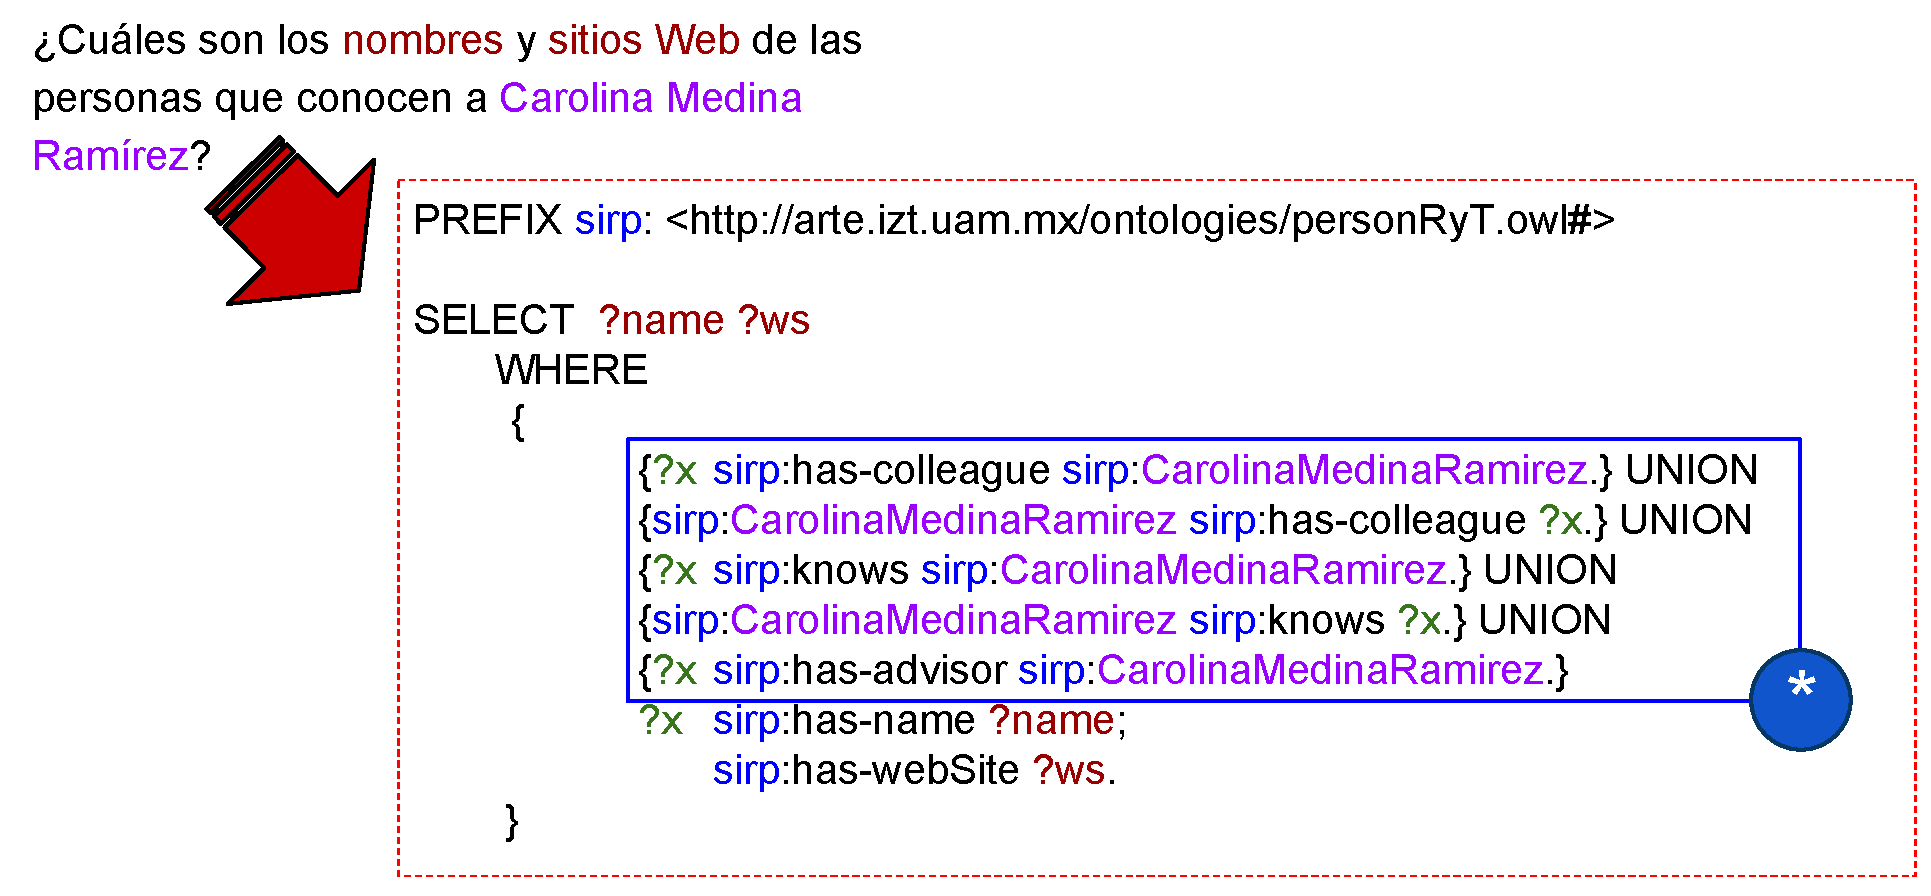
\includegraphics[scale=0.32]{q2rqlSR}
	\end{figure}
	
%	\begin{block}{Actividades}
%	\begin{enumerate}
%	\item \justifying Identificar las preguntas en lenguaje natural.
%	\item \justifying Transformar las preguntas a una consultas SPARQL.
%	\item \justifying Ejecutar las consultas mediante un motor de b�squeda SPARQL.
%	\end{enumerate}
%	\end{block}

\end{frame}

%%%%%%%%%%%%%%%%%%%%%%%%%%%%%%%%%%%%%%%%%%%%%%%%%%%%%%%%%%%%%%%%%%%%%%%%%%%%%%
\subsubsection{B�squeda + Inferencia}
\begin{frame}[allowframebreaks]
	\frametitle{Uso de inferencia}
		
	\begin{figure}
	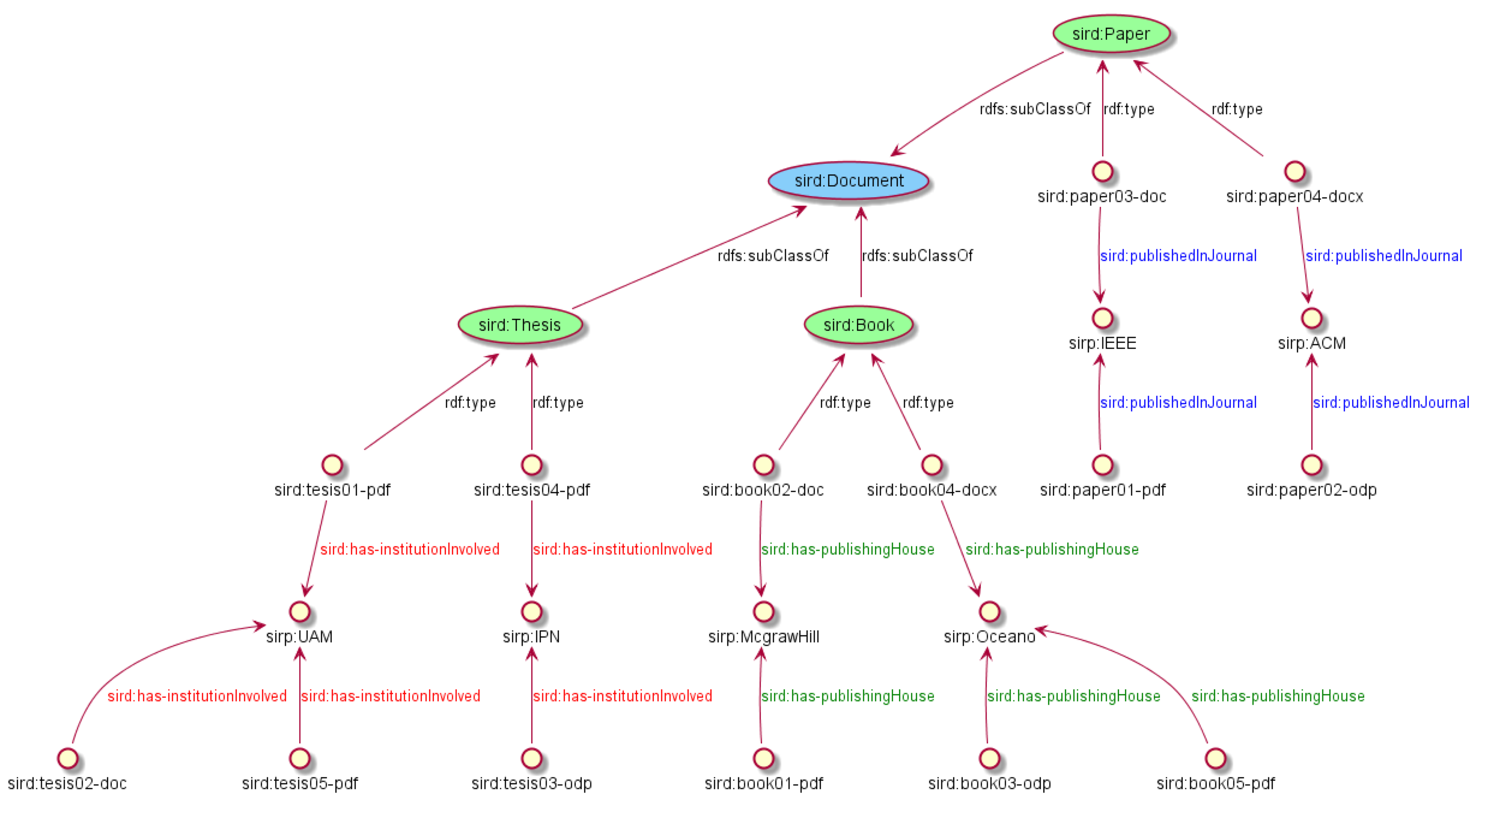
\includegraphics[scale=0.3]{grafoSR}
	\caption{Grafo RDF sin inferencia}
	\end{figure}
	%%%%%%%%%%%%%%%%%%%%%%%%%%%%%%%%%%%
	
	\begin{figure}[htbp]
	\centering
	\subfigure[Consulta sin inferencia]{
	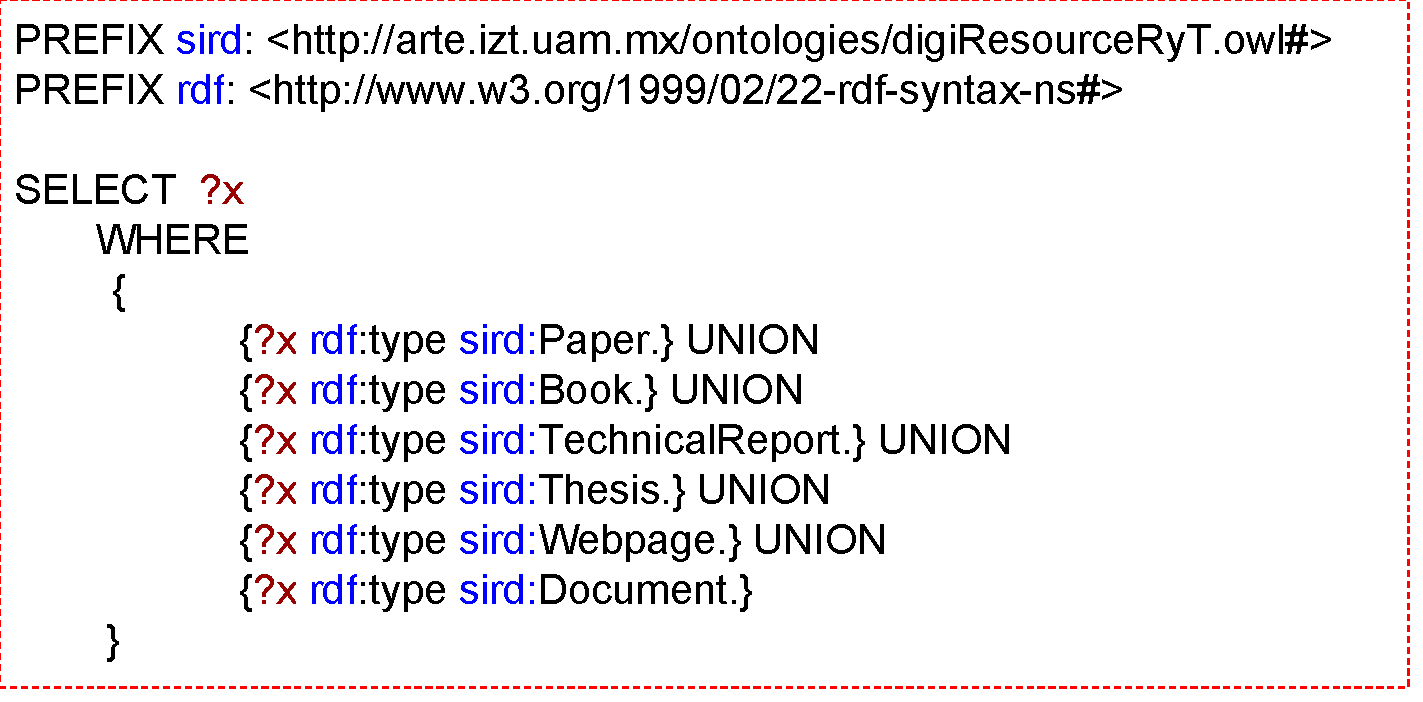
\includegraphics[scale=0.25]{consultaGrafo} 
	}
	\subfigure[Resultados de la consulta]{
	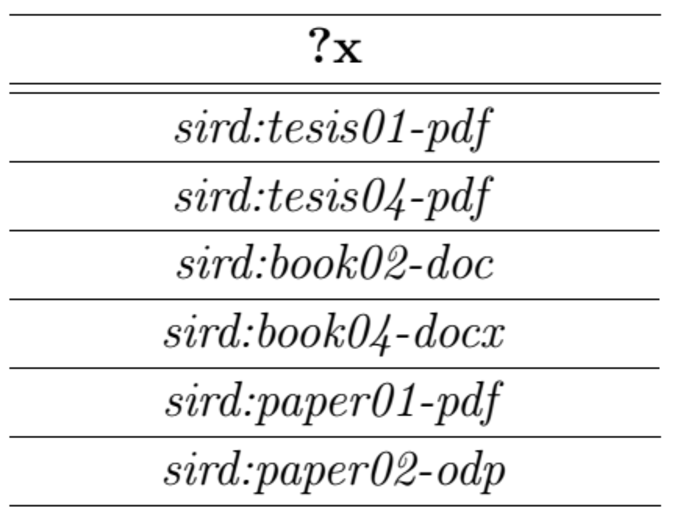
\includegraphics[scale=0.28]{RespQrySI} 
	}
	\end{figure}
	%%%%%%%%%%%%%%%%%%%%%%%%%%%%%%%%%%%
	
	\begin{figure}
	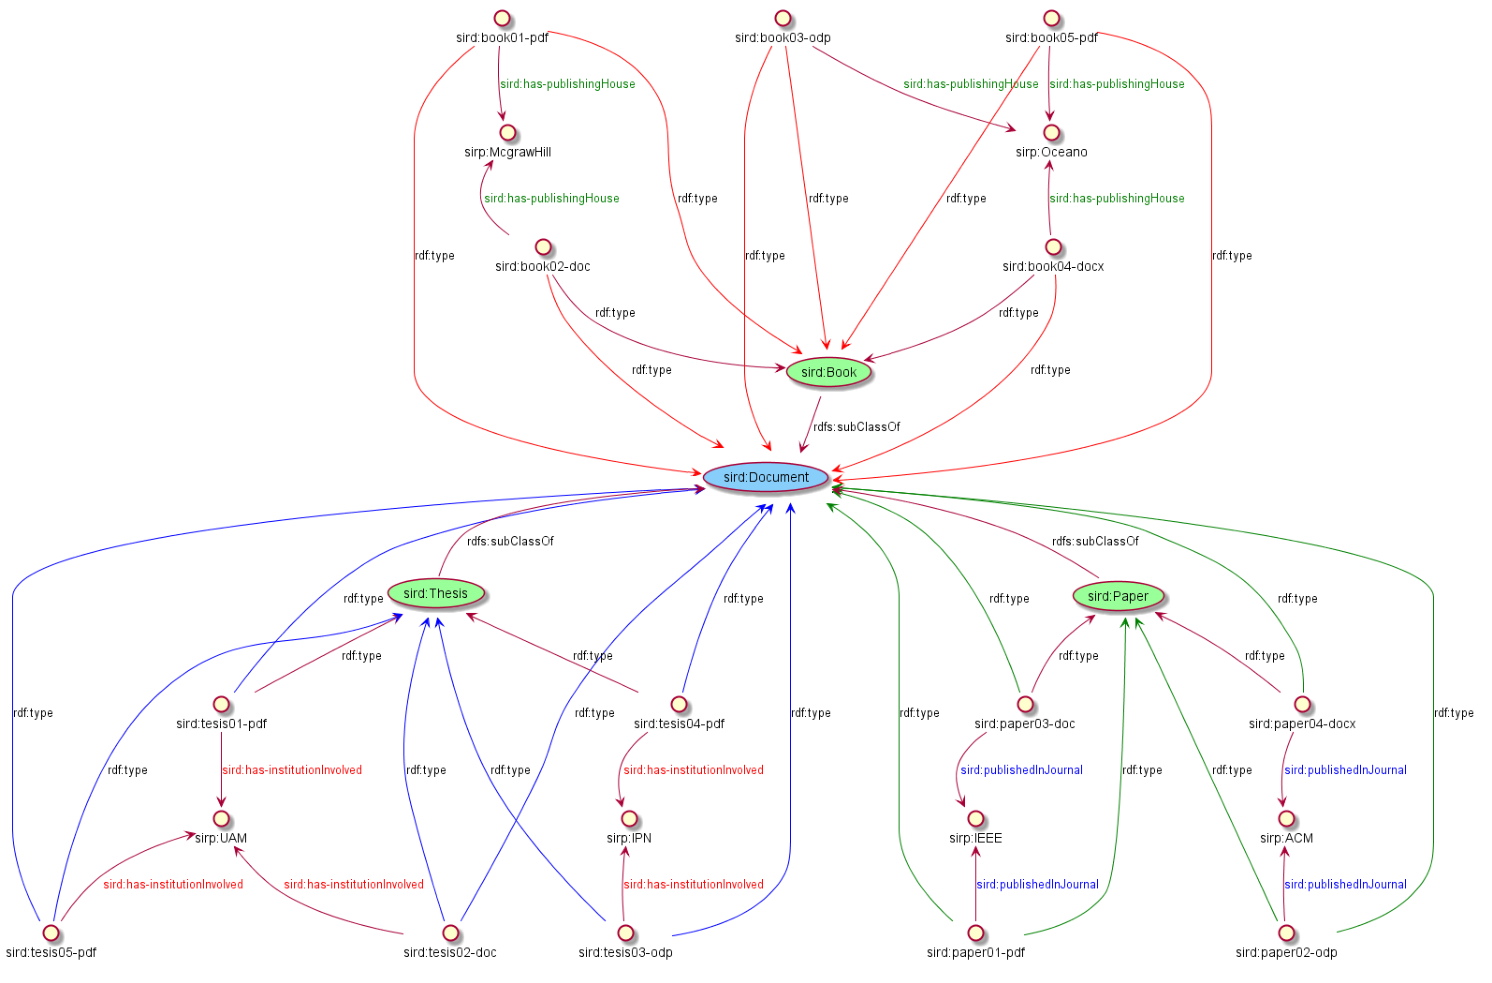
\includegraphics[scale=0.37]{grafoCR}
	\caption{Grafo RDF con inferencia}
	\end{figure}	
	%%%%%%%%%%%%%%%%%%%%%%%%%%%%%%%%%%%
\end{frame}

\subsubsection{Uso de inferencia IV}
\begin{frame}
	\frametitle{Uso de inferencia IV}
	\begin{figure}[htbp]
	\centering
	\subfigure[Consulta con inferencia]{
	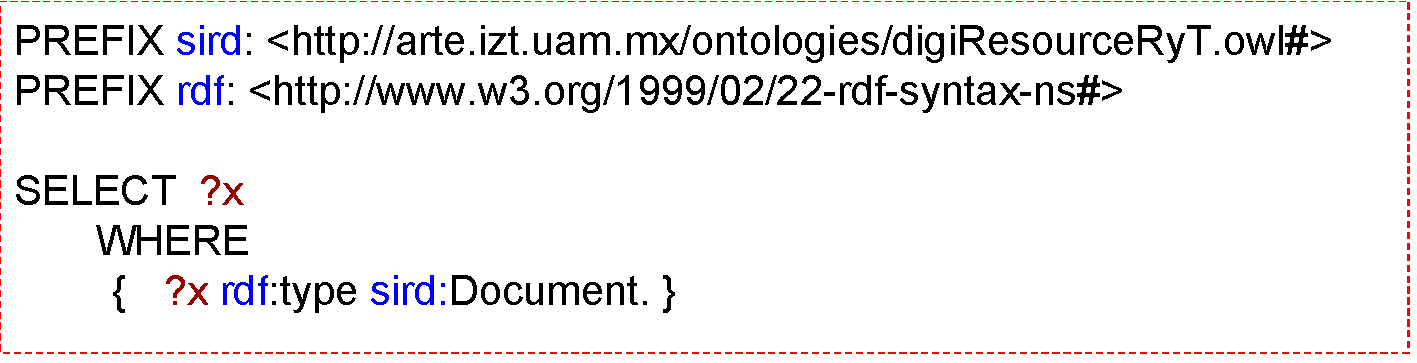
\includegraphics[scale=0.25]{consSimpGrafo} 
	}
	\subfigure[Resultados de la consulta]{
	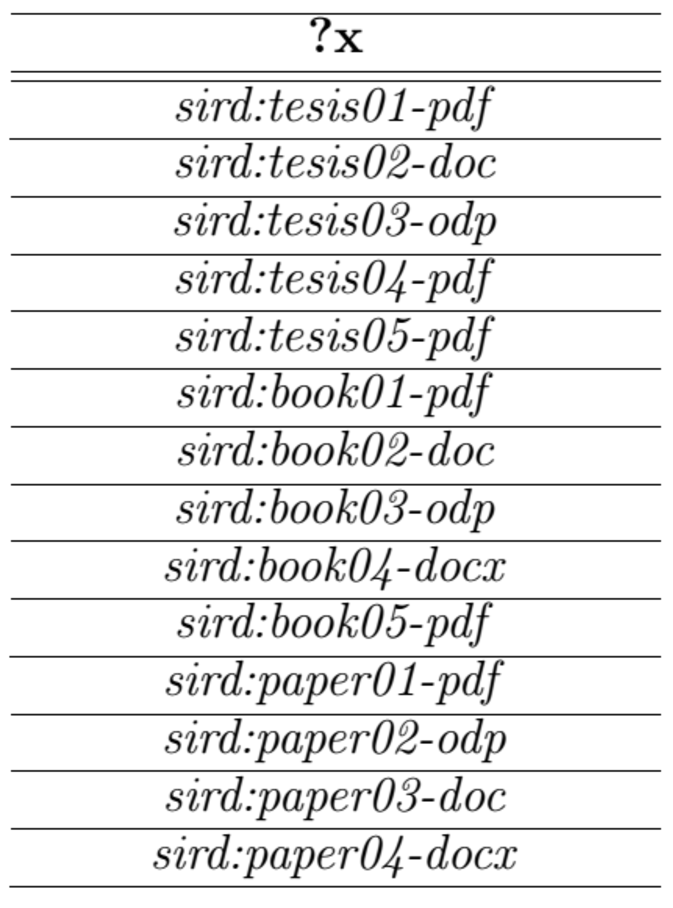
\includegraphics[scale=0.28]{RespQryCI} 
	}
	\end{figure}
\end{frame}
\chapter{Prototipo}
\label{cap:piu}
%%No solo basta con un razonador también se requiere un modulo integrador de la información que transforme las consultas de los usuarios expresadas en lenguaje natural, a lenguaje que sea interpretado por el razonador. Además este integrador es el encargado de regresar los enlaces y los datos del recurso. De esta manera el motor de búsqueda queda de la siguiente manera:

%%Para llevar acabo está integración de la información es necesario un prototipo que satisfaga más eficientemente las consultas que escribe el usuario. De esta manera es necesario un análisis documental y técnico de los módulos de Anotaciones, Ontología de Dominio y Razonadores. Con la finalidad de tener una propuesta de sistema con las últimas novedades hechas en búsqueda y recuperación de la información basada en la semántica de los recursos.

%%se requiere proporcionar interfaces fáciles de usar, para simplificar a los miembros el proceso de generación de anotaciones y colocar en contexto su trabajo.  Un buen enfoque para un sistema de anotaciones es aquel donde se maneja una única interfaz, y es en esta donde los usuarios crean, modifican y comparten sus anotaciones.

%%La interfaz debe tener ..., para que los usuarios estructuren sus consulta, capturando los valores que desean buscar. En la interfaz debe proporcionar un navegador entre personas, documentos, multimedia, para que los usuarios que no tienen algún conocimiento previo de las personas y recursos digitales, puedan tener una vision general de la información de los recursos.

%%La interfaz debe permitir hacer las siguientes actividades a los usuarios:
%%•	Login.
%%•	Navegar entre personas.
%%o	Filtrar por ocupación.
%%o	Mostrar la información más detallada de una persona.
%%o	Búsqueda Avanzada de las personas.
%%•	Navegar entre documentos.
%%o	Filtrar por clase de documento.
%%o	Mostrar la información más detallada de un documento.
%%o	Búsqueda Avanzada de documentos.
%%•	Navegar entre multimedia.
%%o	Filtrar por clase multimedia.
%%o	Mostrar la información más detallada de un recurso multimedia.
%%o	Búsqueda Avanzada de recursos multimedia.
%%•	Búsqueda en todos los recursos de información por información semejante.

%%Las distintas aplicaciones que hay pueden ser elaboradas para Windows, Linux, Macs, u otros sistemas operativos, y también se pueden tener distintas versiones del mismo sistema para poder trabajar entre los distintos sistemas operativos. Lo ideal es que sin importar cual sea el sistema operativo el usuario pueda realizar sus anotaciones semánticas, para logara esto se puede emplear una aplicación web o aplicaciones elaboradas en java.
%%Si se emplea una aplicación web no es necesario instalar algún software extra, solo basta que el usuario acceda utilizando su navegador web de preferencia y comience el proceso de creación de anotaciones semánticas.

%%Por otro lado al usar una aplicación basada en Java, es necesario tener Java Development Kit (JDK) que es independiente de la plataforma, para tener un entorno amigable al usuario.

%%Finalmente, los usuarios necesitan una interfaz de usuario, para la consulta de información de las tripletas. Nosotros proponemos una interfaz amigable que sea accesible vía Web. De esta manera, los usuarios no instalan ningún componente y simplemente acceden a la página Web del sistema.
%%La interfaz al ser accesible vía Web, requiere ser instalada en un servidor Web. Para tomar la decisión sobre qué servidor es el apropiado para la interfaz. Nosotros debemos tomar en cuenta, el lenguaje de implementación del triplestore. Si el lenguaje es PHP9, entonces, podemos emplear un servidor HTTP Apache10. En otro caso, si el lenguaje es Java11 y permite implementar Servlet, entonces el servidor es Apache Tomcat12. 



\section{Referencias}
\begin{frame}[allowframebreaks]
\frametitle{Referencias}
\begin{scriptsize} \bibliographystyle{apalike}
\justifying \bibliography{bibliografia}\end{scriptsize}
\end{frame}

\end{document}
